\documentclass[11pt,a4paper]{report}


\usepackage[utf8]{inputenc}
\usepackage[T1]{fontenc}
\usepackage[margin=1in]{geometry}
\usepackage{xcolor}
\usepackage{listings}
\usepackage{fancyhdr}
\usepackage{titlesec}
\usepackage{hyperref}
\usepackage{tcolorbox}
\usepackage{graphicx}
\usepackage{enumitem}
\usepackage{tabularx}
\usepackage{booktabs}
\usepackage{amsmath}
\usepackage{tikz}
\usetikzlibrary{arrows.meta, positioning, shapes.geometric}
\usepackage{float}
\usepackage{parskip}


\definecolor{codebg}{RGB}{245,245,245}
\definecolor{codekeyword}{RGB}{0,0,180}
\definecolor{codecomment}{RGB}{100,100,100}
\definecolor{codestring}{RGB}{163,21,21}
\definecolor{titleblue}{RGB}{20,60,120}
\definecolor{notebg}{RGB}{235,245,255}
\definecolor{warnbg}{RGB}{255,240,235}


\lstdefinestyle{cstyle}{
    backgroundcolor=\color{codebg},
    commentstyle=\color{codecomment}\itshape,
    keywordstyle=\color{codekeyword}\bfseries,
    stringstyle=\color{codestring},
    basicstyle=\ttfamily\footnotesize,
    breakatwhitespace=false,
    breaklines=true,
    captionpos=b,
    keepspaces=true,
    numbers=left,
    numbersep=8pt,
    numberstyle=\tiny\color{gray},
    showspaces=false,
    showstringspaces=false,
    showtabs=false,
    tabsize=4,
    frame=single,
    rulecolor=\color{gray!40},
    xleftmargin=15pt,
    language=C
}
\lstset{style=cstyle}

\lstdefinestyle{bashstyle}{
    backgroundcolor=\color{codebg},
    basicstyle=\ttfamily\footnotesize,
    breaklines=true,
    frame=single,
    rulecolor=\color{gray!40},
    xleftmargin=15pt,
    language=bash,
    commentstyle=\color{codecomment}\itshape,
    keywordstyle=\color{codekeyword}\bfseries,
    stringstyle=\color{codestring},
}


\newtcolorbox{note}{
    colback=notebg, colframe=titleblue!60, boxrule=0.5pt,
    left=6pt, right=6pt, top=4pt, bottom=4pt,
    title=\textbf{Note}, fonttitle=\bfseries, coltitle=titleblue
}
\newtcolorbox{warnbox}{
    colback=warnbg, colframe=orange!70!black, boxrule=0.5pt,
    left=6pt, right=6pt, top=4pt, bottom=4pt,
    title=\textbf{Common Pitfall}, fonttitle=\bfseries, coltitle=orange!70!black
}


\pagestyle{fancy}
\fancyhf{}
\fancyhead[L]{\small\leftmark}
\fancyhead[R]{\small\thepage}
\renewcommand{\headrulewidth}{0.4pt}


\titleformat{\chapter}[display]
  {\normalfont\huge\bfseries\color{titleblue}}
  {\chaptertitlename\ \thechapter}{20pt}{\Huge}
\titleformat{\section}
  {\normalfont\Large\bfseries\color{titleblue}}
  {\thesection}{1em}{}
\titleformat{\subsection}
  {\normalfont\large\bfseries\color{titleblue!80}}
  {\thesubsection}{1em}{}


\hypersetup{
    colorlinks=true,
    linkcolor=titleblue,
    citecolor=titleblue,
    urlcolor=titleblue,
    pdftitle={Protocols Implementation: HTTP and Gopher from Scratch in C},
    pdfauthor={Mohammed Bakr},
    pdfsubject={Systems Programming, Networking, Sockets},
}

\newcommand{\inlinecode}[1]{\texttt{\textcolor{titleblue!80}{#1}}}

\title{
    \vspace{-2cm}
    {\Huge \textbf{Protocols Implementation}}\\[0.5em]
    {\Large HTTP and Gopher Protocols from Scratch in C}\\[1em]
    {\large A Line-by-Line Technical Walkthrough}
}
\author{Mohammed Bakr}
\date{\today}

\begin{document}

\maketitle
\thispagestyle{empty}

\begin{center}
\vspace{2cm}
\begin{tcolorbox}[colback=notebg, colframe=titleblue!60, width=0.8\textwidth, boxrule=0.5pt]
\textbf{Repository:} \url{https://github.com/MohammedBakr1/Protocols_Implementation}\\
\textbf{Language:} C (C11 standard)\\
\textbf{Platform:} Linux (POSIX sockets API)\\
\textbf{License:} MIT
\end{tcolorbox}
\end{center}

\newpage
\thispagestyle{empty}
\tableofcontents

\newpage

\chapter{Introduction}

\section{Purpose of This Project}

This project implements two application-layer network protocols entirely from scratch in C, using nothing but the raw POSIX sockets API:

\begin{itemize}
    \item \textbf{Gopher} (RFC 1436) --- a minimalist document-retrieval protocol from 1991.
    \item \textbf{HTTP/1.1} (a practical subset) --- the protocol underlying the modern web.
\end{itemize}

For each protocol, both a \textbf{server} and a \textbf{client} are implemented. No external networking libraries are used; every byte sent or received passes through hand-written code that calls directly into the operating system's socket layer (\inlinecode{socket()}, \inlinecode{bind()}, \inlinecode{listen()}, \inlinecode{accept()}, \inlinecode{connect()}, \inlinecode{send()}, \inlinecode{recv()}).

\section{Why These Two Protocols Together}

Gopher and HTTP were chosen deliberately as a pair, not arbitrarily:

\begin{itemize}
    \item \textbf{Gopher is almost the simplest possible TCP application protocol.} A request is a single line of text; a response is raw bytes followed by connection closure. There are no headers, no status codes, and no explicit content length. This makes it an ideal first target: it forces you to master the TCP connection lifecycle (\inlinecode{accept}/\inlinecode{connect}, \inlinecode{recv} loops, \inlinecode{send} loops, closing sockets) without the added complexity of message framing.

    \item \textbf{HTTP adds exactly the complexity that Gopher lacks.} Once the TCP fundamentals are solid, HTTP introduces the next layer of concepts that essentially every real-world protocol needs: structured request/response lines, key--value headers, explicit content-length framing, and status codes. Implementing HTTP after Gopher means each new concept is introduced in isolation, rather than all at once.
\end{itemize}

The result is a natural progression: Chapter~\ref{chap:gopher-protocol} onward builds the simple case, and Chapter~\ref{chap:http-protocol} onward builds on top of the same socket primitives to handle the harder case.

\section{Learning Goals}

By the end of working through this project and this document, the reader should be able to:

\begin{enumerate}
    \item Explain the full lifecycle of a TCP server socket (\inlinecode{socket} $\to$ \inlinecode{bind} $\to$ \inlinecode{listen} $\to$ \inlinecode{accept}) and a TCP client socket (\inlinecode{socket} $\to$ \inlinecode{connect}).
    \item Explain why \inlinecode{recv()} and \inlinecode{send()} do not guarantee delivering or accepting all requested bytes in a single call, and why loops are required around both.
    \item Implement a simple line-based protocol (Gopher) that relies on connection closure to signal the end of a message.
    \item Implement a framed protocol (HTTP) that relies on an explicit \inlinecode{Content-Length} header, including correctly separating headers from body in a byte stream.
    \item Understand basic server-side input validation (e.g.\ path traversal protection) and why client-side behavior (e.g.\ URL normalization in \texttt{curl}) cannot be relied upon for security.
    \item Build and run all of the above on a Linux system, including troubleshooting the most common pitfalls (buffering, working directory issues, background process management).
\end{enumerate}

\section{Prerequisites}

The reader is assumed to have:
\begin{itemize}
    \item Working knowledge of C (pointers, structs, manual memory management with \inlinecode{malloc}/\inlinecode{free}).
    \item Basic familiarity with the command line on Linux.
    \item No prior networking experience is assumed --- Chapter~\ref{chap:networking-fundamentals} builds the necessary background from first principles.
\end{itemize}

\section{Document Structure}

\begin{itemize}
    \item \textbf{Chapter~\ref{chap:networking-fundamentals}} builds the conceptual foundation: what a socket is, the TCP three-way handshake, byte ordering, and blocking I/O.
    \item \textbf{Chapter~\ref{chap:project-structure}} gives a bird's-eye view of the repository layout.
    \item \textbf{Chapter~\ref{chap:socket-utils}} walks through the shared utility library used by every server and client in the project.
    \item \textbf{Chapters~\ref{chap:gopher-protocol}--\ref{chap:gopher-client}} cover the Gopher protocol, server, and client in full detail.
    \item \textbf{Chapters~\ref{chap:http-protocol}--\ref{chap:http-client}} cover HTTP in the same depth.
    \item \textbf{Chapter~\ref{chap:build-system}} explains the \inlinecode{Makefile}.
    \item \textbf{Chapter~\ref{chap:running-on-linux}} is a practical, copy-pasteable guide to building and running everything on Linux.
    \item \textbf{Chapter~\ref{chap:testing}} documents how each component was verified to work correctly.
    \item \textbf{Chapter~\ref{chap:limitations}} is an honest account of what this implementation deliberately does \emph{not} handle, and what a production-grade version would need to add.
\end{itemize}

\chapter{Networking Fundamentals}
\label{chap:networking-fundamentals}

This chapter builds the conceptual vocabulary used throughout the rest of the document. Readers already comfortable with sockets, TCP, and byte ordering may skip to Chapter~\ref{chap:project-structure}.

\section{What Is a Socket?}

A \textbf{socket} is an operating-system abstraction representing one endpoint of a bidirectional communication channel. From the perspective of a C program, a socket behaves much like a file: the kernel hands back an integer \textbf{file descriptor} (fd), and the program reads from and writes to that descriptor using system calls. The key difference is that instead of reading/writing bytes to a file on disk, the bytes travel across a network (or, in the case of \texttt{localhost}, through a loopback interface without ever leaving the machine).

Every socket used in this project is created with:

\begin{lstlisting}[style=cstyle]
int fd = socket(AF_INET, SOCK_STREAM, 0);
\end{lstlisting}

\begin{itemize}
    \item \inlinecode{AF\_INET} selects the IPv4 address family.
    \item \inlinecode{SOCK\_STREAM} selects TCP: a connection-oriented, reliable, ordered byte stream.
    \item The third argument (\inlinecode{0}) lets the kernel pick the default protocol for the given family/type combination, which for \inlinecode{SOCK\_STREAM} is always TCP.
\end{itemize}

\begin{note}
This project exclusively uses TCP (\inlinecode{SOCK\_STREAM}). The alternative, \inlinecode{SOCK\_DGRAM} (UDP), provides no ordering or delivery guarantees and is not used here. Both HTTP and Gopher are defined as TCP protocols.
\end{note}

\section{The TCP Connection Lifecycle}

\subsection{Server Side}

A TCP server follows a strict sequence of system calls:

\begin{enumerate}
    \item \textbf{\inlinecode{socket()}} --- create an unbound, unconnected socket.
    \item \textbf{\inlinecode{bind()}} --- associate the socket with a specific local IP address and port number.
    \item \textbf{\inlinecode{listen()}} --- mark the socket as passive (willing to accept incoming connections), and specify a backlog queue size.
    \item \textbf{\inlinecode{accept()}} --- block until a client connects, then return a \emph{new} file descriptor representing that specific connection. The original listening socket remains open and can accept further connections.
    \item \textbf{\inlinecode{recv()} / \inlinecode{send()}} --- exchange data with the connected client, using the fd returned by \inlinecode{accept()}, not the listening fd.
    \item \textbf{\inlinecode{close()}} --- close the per-connection fd once the exchange is finished.
\end{enumerate}

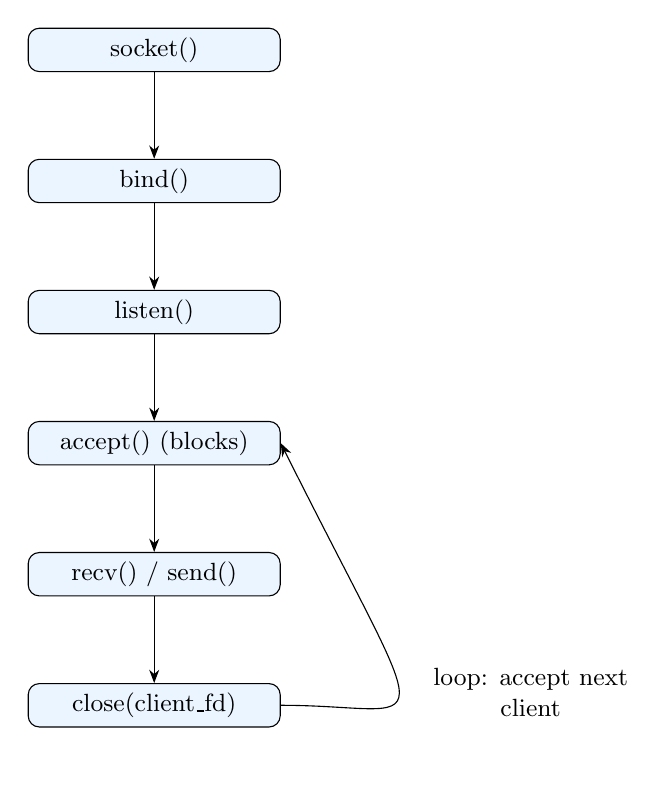
\begin{tikzpicture}[node distance=1.1cm, every node/.style={font=\small}]
    \node[draw, rectangle, rounded corners, fill=notebg, minimum width=3.2cm] (s1) {socket()};
    \node[draw, rectangle, rounded corners, fill=notebg, minimum width=3.2cm, below=of s1] (s2) {bind()};
    \node[draw, rectangle, rounded corners, fill=notebg, minimum width=3.2cm, below=of s2] (s3) {listen()};
    \node[draw, rectangle, rounded corners, fill=notebg, minimum width=3.2cm, below=of s3] (s4) {accept() (blocks)};
    \node[draw, rectangle, rounded corners, fill=notebg, minimum width=3.2cm, below=of s4] (s5) {recv() / send()};
    \node[draw, rectangle, rounded corners, fill=notebg, minimum width=3.2cm, below=of s5] (s6) {close(client\_fd)};

    \draw[-Stealth] (s1) -- (s2);
    \draw[-Stealth] (s2) -- (s3);
    \draw[-Stealth] (s3) -- (s4);
    \draw[-Stealth] (s4) -- (s5);
    \draw[-Stealth] (s5) -- (s6);
    \draw[-Stealth] (s6.east) .. controls +(2,0) and +(2,-4) .. (s4.east)
        node[midway, right, xshift=0.3cm] {\parbox{2.5cm}{\centering loop: accept next client}};
\end{tikzpicture}

\subsection{Client Side}

A client's sequence is much shorter:

\begin{enumerate}
    \item \textbf{\inlinecode{socket()}} --- create the socket.
    \item \textbf{\inlinecode{connect()}} --- initiate the TCP three-way handshake with a specific server address and port. This call blocks until the handshake completes (or fails).
    \item \textbf{\inlinecode{send()} / \inlinecode{recv()}} --- exchange data.
    \item \textbf{\inlinecode{close()}} --- close the connection.
\end{enumerate}

\section{The TCP Three-Way Handshake}

Although the handshake itself is handled transparently by the kernel when \inlinecode{connect()} and \inlinecode{accept()} are called, understanding it explains why these calls can block and occasionally fail:

\begin{enumerate}
    \item \textbf{SYN}: the client sends a segment requesting synchronization.
    \item \textbf{SYN-ACK}: the server acknowledges and sends its own synchronization request.
    \item \textbf{ACK}: the client acknowledges the server's request.
\end{enumerate}

Only after this exchange completes does \inlinecode{accept()} on the server return a usable connected file descriptor, and does \inlinecode{connect()} on the client return successfully.

\section{Byte Order: Why \texttt{htons()} Exists}

Different CPU architectures store multi-byte integers in memory in different orders:

\begin{itemize}
    \item \textbf{Little-endian} (e.g.\ x86, x86-64): the least significant byte is stored first.
    \item \textbf{Big-endian} (e.g.\ many older RISC systems, and network protocols by convention): the most significant byte is stored first.
\end{itemize}

Network protocols standardize on big-endian, historically called \textbf{network byte order}. Because a client and server may run on machines with different native (\textbf{host}) byte orders, port numbers and IP addresses must be explicitly converted before being placed into a \inlinecode{struct sockaddr\_in}. This project uses:

\begin{lstlisting}[style=cstyle]
addr.sin_port = htons(port);
\end{lstlisting}

\inlinecode{htons} stands for \textbf{h}ost \textbf{to} \textbf{n}etwork, \textbf{s}hort (16-bit). The corresponding reverse conversion is \inlinecode{ntohs}. For 32-bit values (such as IPv4 addresses), the analogous functions are \inlinecode{htonl} and \inlinecode{ntohl}.

\begin{warnbox}
Forgetting \inlinecode{htons()} is a classic bug: on a little-endian machine, binding to port 8080 (\texttt{0x1F90}) without conversion would actually bind to port \texttt{0x901F} = 36895. The code would compile and run without error, but the server would listen on the wrong port.
\end{warnbox}

\section{Blocking I/O and Partial Reads/Writes}
\label{sec:partial-io}

This is the single most important practical lesson in this project, and the reason the shared utility library (Chapter~\ref{chap:socket-utils}) exists at all.

\subsection{\texttt{recv()} May Return Fewer Bytes Than Requested}

When a program calls \inlinecode{recv(fd, buffer, 4096, 0)}, it is asking the kernel for \emph{up to} 4096 bytes. The kernel is free to return anywhere from 1 byte to 4096 bytes in a single call, depending on how much data has arrived and been buffered so far. TCP is a \emph{byte stream}, not a message-based protocol: it makes no promise that the boundaries of your \inlinecode{send()} calls on one side will match the boundaries of your \inlinecode{recv()} calls on the other side.

Consequently, any code that assumes ``one \inlinecode{recv()} call = one complete message'' is incorrect in general, even though it may appear to work reliably in local testing (where messages are small and the loopback interface rarely fragments them).

\subsection{\texttt{send()} May Send Fewer Bytes Than Requested}

Symmetrically, \inlinecode{send(fd, buffer, len, 0)} is permitted to transmit fewer than \inlinecode{len} bytes and return the actual number sent. This typically happens when the kernel's internal send buffer is full. Code that ignores the return value of \inlinecode{send()} silently truncates its own output under load.

\subsection{The Standard Fix: Loop Until Done}

The correct pattern for both directions is a loop:

\begin{lstlisting}[style=cstyle]
size_t sent_total = 0;
while (sent_total < len) {
    ssize_t n = send(fd, buf + sent_total, len - sent_total, 0);
    if (n < 0) { /* handle error */ }
    sent_total += (size_t)n;
}
\end{lstlisting}

This project implements exactly this pattern once, in \inlinecode{send\_all()} (Chapter~\ref{chap:socket-utils}), and reuses it everywhere data needs to be sent reliably.

\section{Signaling the End of a Message}

Because TCP is a raw byte stream with no built-in concept of ``message boundaries,'' every application-layer protocol must define its own way of telling the receiver when a logical message is complete. This project's two protocols use the two most common strategies, which is precisely why they were chosen together:

\begin{itemize}
    \item \textbf{Connection closure} (used by Gopher): the sender simply closes the connection once done. The receiver knows the message is complete when \inlinecode{recv()} returns \texttt{0} (end-of-file on the socket).
    \item \textbf{Explicit length framing} (used by HTTP): the sender includes a \inlinecode{Content-Length} header stating exactly how many body bytes follow the headers. The receiver first finds the end of the headers (the sequence \texttt{"\textbackslash r\textbackslash n\textbackslash r\textbackslash n"}), then reads exactly that many additional bytes.
\end{itemize}

Both strategies are explored in depth in their respective protocol chapters.

\chapter{Project Structure}
\label{chap:project-structure}

\section{Repository Layout}

\begin{lstlisting}[style=bashstyle, numbers=none]
Protocols_Implementation/
|-- common/
|   |-- socket_utils.h      Shared socket helper declarations
|   `-- socket_utils.c      Shared socket helper implementation
|-- gopher/
|   |-- gopher_server.c     Gopher server
|   |-- gopher_client.c     Gopher client
|   `-- gopher_root/        Sample files served by the Gopher server
|       |-- README
|       `-- about.txt
|-- http/
|   |-- http_server.c       HTTP server
|   |-- http_client.c       HTTP client
|   `-- www/                Sample files served by the HTTP server
|       |-- index.html
|       `-- about.txt
|-- docs/                   This LaTeX document and its compiled PDF
|   |-- main.tex
|   |-- chapters/
|   `-- Protocols_Implementation.pdf
|-- Makefile
|-- README.md
`-- LICENSE
\end{lstlisting}

\section{Design Rationale}

\subsection{Why a Shared \texttt{common/} Module?}

Both protocols' servers and clients need to perform the same low-level operations: create a listening socket, connect as a client, reliably send a buffer, and (for Gopher) read until the peer closes the connection. Rather than duplicating this logic four times, it is factored into \inlinecode{common/socket\_utils.c}, and every other file includes its header and links against its object file. This is standard C practice: a small, focused, reusable module with a clear interface (declared in the \texttt{.h} file) and a hidden implementation (in the \texttt{.c} file).

\subsection{Why Separate Directories per Protocol?}

Keeping \texttt{gopher/} and \texttt{http/} as separate directories, each with its own sample-content folder (\texttt{gopher\_root/} and \texttt{www/}), mirrors how real servers are typically organized: application code separate from the content it serves. It also keeps the two protocol implementations visually and organizationally independent, which matters for a project whose explicit purpose is pedagogical comparison between the two.

\subsection{Four Independent \texttt{main()} Functions}

This project intentionally builds four separate executables rather than one combined program with subcommands:

\begin{center}
\begin{tabularx}{\textwidth}{l l X}
\toprule
\textbf{Executable} & \textbf{Source file} & \textbf{Role} \\
\midrule
\texttt{gopher\_server} & \texttt{gopher/gopher\_server.c} & Listens on TCP port 7070, serves Gopher selectors \\
\texttt{gopher\_client} & \texttt{gopher/gopher\_client.c} & Connects to a Gopher server and prints the response \\
\texttt{http\_server} & \texttt{http/http\_server.c} & Listens on TCP port 8080, serves files over HTTP/1.1 \\
\texttt{http\_client} & \texttt{http/http\_client.c} & Connects to an HTTP server, sends a GET request, parses the response \\
\bottomrule
\end{tabularx}
\end{center}

Each has its own \inlinecode{int main(int argc, char *argv[])}. This is why, when importing the project into an IDE such as Code::Blocks, it must be imported as a \emph{Makefile project} rather than a single ``C project'' --- a normal single-target C project expects exactly one \inlinecode{main()} across all its source files, and would fail to link with four.

\chapter{The Shared Socket Utility Library}
\label{chap:socket-utils}

This chapter examines \texttt{common/socket\_utils.h} and \texttt{common/socket\_utils.c} in full detail. Every other C file in the project depends on this module, so a thorough understanding of it is a prerequisite for the rest of the document.

\section{The Header File: \texttt{socket\_utils.h}}

\begin{lstlisting}[style=cstyle]
#ifndef SOCKET_UTILS_H
#define SOCKET_UTILS_H

int create_server_socket(int port, int backlog);
int connect_to_server(const char *host, int port);
char *read_until_close(int fd, size_t *out_len);
int send_all(int fd, const char *buf, size_t len);

#endif
\end{lstlisting}

\subsection{Include Guards}

The \inlinecode{\#ifndef} / \inlinecode{\#define} / \inlinecode{\#endif} triplet is a standard \textbf{include guard}. If this header is accidentally included more than once within the same translation unit (which can happen indirectly through chains of includes), the guard prevents the compiler from seeing duplicate declarations, which would otherwise be a compile error.

\subsection{The Four Declared Functions}

\begin{center}
\begin{tabularx}{\textwidth}{l X}
\toprule
\textbf{Function} & \textbf{Purpose} \\
\midrule
\inlinecode{create\_server\_socket} & Performs \inlinecode{socket}, \inlinecode{setsockopt}, \inlinecode{bind}, and \inlinecode{listen} in one call; returns a ready-to-\inlinecode{accept} listening file descriptor. \\
\inlinecode{connect\_to\_server} & Performs \inlinecode{getaddrinfo}, \inlinecode{socket}, and \inlinecode{connect}; returns a connected file descriptor. \\
\inlinecode{read\_until\_close} & Reads from a socket in a loop until the peer closes the connection (EOF), dynamically growing a heap buffer as needed. \\
\inlinecode{send\_all} & Sends an entire buffer over a socket, looping as necessary to handle partial writes (see Section~\ref{sec:partial-io}). \\
\bottomrule
\end{tabularx}
\end{center}

\section{The Implementation File: \texttt{socket\_utils.c}}

\subsection{Feature Test Macro and Includes}

\begin{lstlisting}[style=cstyle]
#define _POSIX_C_SOURCE 200809L
#include <stdio.h>
#include <stdlib.h>
#include <string.h>
#include <unistd.h>
#include <errno.h>
#include <sys/socket.h>
#include <netinet/in.h>
#include <arpa/inet.h>
#include <netdb.h>
#include "socket_utils.h"
\end{lstlisting}

The project is compiled with \inlinecode{-std=c11}, which tells GCC to expose only strictly-standard C library features and hide POSIX-specific extensions such as \inlinecode{getaddrinfo}. Defining \inlinecode{\_POSIX\_C\_SOURCE 200809L} \emph{before any header is included} explicitly requests the POSIX.1-2008 feature set, making functions like \inlinecode{getaddrinfo} and \inlinecode{gai\_strerror} visible again. This macro must appear before the very first \inlinecode{\#include} line to take effect correctly.

\subsection{\texttt{create\_server\_socket}}

\begin{lstlisting}[style=cstyle]
int create_server_socket(int port, int backlog) {
    int server_fd = socket(AF_INET, SOCK_STREAM, 0);
    if (server_fd < 0) {
        perror("socket");
        return -1;
    }
\end{lstlisting}

Creates a TCP/IPv4 socket. \inlinecode{perror} prints a human-readable description of \inlinecode{errno} (the last system-call error code) prefixed with the given string, e.g. \texttt{socket: Too many open files}.

\begin{lstlisting}[style=cstyle]
    int opt = 1;
    if (setsockopt(server_fd, SOL_SOCKET, SO_REUSEADDR, &opt, sizeof(opt)) < 0) {
        perror("setsockopt");
        close(server_fd);
        return -1;
    }
\end{lstlisting}

\inlinecode{SO\_REUSEADDR} allows the socket to bind to a port that is still nominally occupied by a recently-closed connection lingering in the \texttt{TIME\_WAIT} state. Without this option, restarting the server immediately after stopping it often fails with \texttt{Address already in use}, because the kernel reserves the port for a short grace period (typically up to a couple of minutes) to catch any stray packets from the previous connection.

\begin{lstlisting}[style=cstyle]
    struct sockaddr_in addr;
    memset(&addr, 0, sizeof(addr));
    addr.sin_family = AF_INET;
    addr.sin_addr.s_addr = INADDR_ANY;
    addr.sin_port = htons(port);

    if (bind(server_fd, (struct sockaddr *)&addr, sizeof(addr)) < 0) {
        perror("bind");
        close(server_fd);
        return -1;
    }
\end{lstlisting}

\inlinecode{struct sockaddr\_in} describes an IPv4 endpoint (address family, port, IP address). It is zero-initialized with \inlinecode{memset} first as defensive practice, since uninitialized padding bytes in the struct could otherwise contain garbage. \inlinecode{INADDR\_ANY} means ``bind to all available network interfaces on this machine'' (as opposed to a single specific IP). \inlinecode{htons(port)} converts the port number to network byte order, as explained in Section~\ref{sec:partial-io} of the previous chapter. The cast to \inlinecode{struct sockaddr~*} is required because the POSIX sockets API is written in terms of a generic address structure that specific address families (like \inlinecode{sockaddr\_in}) are meant to be cast to and from.

\begin{lstlisting}[style=cstyle]
    if (listen(server_fd, backlog) < 0) {
        perror("listen");
        close(server_fd);
        return -1;
    }

    return server_fd;
}
\end{lstlisting}

\inlinecode{listen} transitions the socket into passive (listening) mode. \inlinecode{backlog} bounds how many fully-established connections may queue up waiting for the program to call \inlinecode{accept()}; if the queue is full, further connection attempts may be refused or delayed by the kernel.

\subsection{\texttt{connect\_to\_server}}

\begin{lstlisting}[style=cstyle]
int connect_to_server(const char *host, int port) {
    struct addrinfo hints, *res;
    memset(&hints, 0, sizeof(hints));
    hints.ai_family = AF_INET;
    hints.ai_socktype = SOCK_STREAM;

    char port_str[16];
    snprintf(port_str, sizeof(port_str), "%d", port);

    int err = getaddrinfo(host, port_str, &hints, &res);
    if (err != 0) {
        fprintf(stderr, "getaddrinfo: %s\n", gai_strerror(err));
        return -1;
    }
\end{lstlisting}

Unlike the server, which always binds to \inlinecode{INADDR\_ANY} (a fixed numeric address), the client must resolve a possibly symbolic host name (e.g.\ \texttt{"localhost"} or \texttt{"example.com"}) into a concrete address. \inlinecode{getaddrinfo} performs this resolution --- including DNS lookups when necessary --- and is the modern, protocol-independent replacement for older functions like \inlinecode{gethostbyname}. It takes the port as a \emph{string}, hence the \inlinecode{snprintf} conversion. On success, \inlinecode{res} points to a linked list of candidate addresses; this project simply uses the first one.

\begin{lstlisting}[style=cstyle]
    int fd = socket(res->ai_family, res->ai_socktype, res->ai_protocol);
    if (fd < 0) {
        perror("socket");
        freeaddrinfo(res);
        return -1;
    }

    if (connect(fd, res->ai_addr, res->ai_addrlen) < 0) {
        perror("connect");
        close(fd);
        freeaddrinfo(res);
        return -1;
    }

    freeaddrinfo(res);
    return fd;
}
\end{lstlisting}

The socket is created using the family/type/protocol values \emph{returned by} \inlinecode{getaddrinfo} rather than hard-coded constants, which keeps the code correct even if \inlinecode{hints} were later relaxed to allow IPv6. \inlinecode{connect} performs the TCP three-way handshake. \inlinecode{freeaddrinfo} releases the linked list allocated by \inlinecode{getaddrinfo}; note it must be called on \emph{every} exit path, including the error paths, to avoid a memory leak.

\subsection{\texttt{read\_until\_close}}

This function implements the Gopher-style ``read until the peer disconnects'' pattern discussed in Section~\ref{sec:partial-io}.

\begin{lstlisting}[style=cstyle]
char *read_until_close(int fd, size_t *out_len) {
    size_t capacity = 4096;
    size_t len = 0;
    char *buf = malloc(capacity);
    if (!buf) return NULL;

    while (1) {
        if (len + 1024 > capacity) {
            capacity *= 2;
            char *new_buf = realloc(buf, capacity);
            if (!new_buf) {
                free(buf);
                return NULL;
            }
            buf = new_buf;
        }
\end{lstlisting}

The buffer starts at 4096 bytes and doubles in size whenever fewer than 1024 bytes of headroom remain. Doubling (rather than growing by a fixed increment) is the standard amortized-growth strategy used by dynamic arrays: it keeps the total number of \inlinecode{realloc} calls logarithmic in the final size, rather than linear.

\begin{warnbox}
If \inlinecode{realloc} fails, the old \inlinecode{buf} pointer is still valid, but the return value \inlinecode{new\_buf} is \inlinecode{NULL}. Overwriting \inlinecode{buf} directly with the result of a failed \inlinecode{realloc} would leak the original allocation. This code correctly checks \inlinecode{new\_buf} before reassigning \inlinecode{buf}.
\end{warnbox}

\begin{lstlisting}[style=cstyle]
        ssize_t n = recv(fd, buf + len, capacity - len - 1, 0);
        if (n < 0) {
            perror("recv");
            free(buf);
            return NULL;
        }
        if (n == 0) {
            break;
        }
        len += (size_t)n;
    }

    buf[len] = '\0';
    if (out_len) *out_len = len;
    return buf;
}
\end{lstlisting}

The read request size is \inlinecode{capacity - len - 1}, deliberately reserving one byte so a null terminator can always be appended afterward, even though the data itself may be binary and the null terminator is mostly a convenience for treating text responses as C strings. \inlinecode{n == 0} is the defining signal of a clean connection close (end-of-file on the socket) and is what allows this function to know when the peer is finished sending. \inlinecode{n < 0} indicates a genuine error (inspect \inlinecode{errno} for the cause).

The caller receives ownership of the heap-allocated buffer and is responsible for calling \inlinecode{free()} on it --- exactly as documented in the header comment.

\subsection{\texttt{send\_all}}

\begin{lstlisting}[style=cstyle]
int send_all(int fd, const char *buf, size_t len) {
    size_t sent_total = 0;
    while (sent_total < len) {
        ssize_t n = send(fd, buf + sent_total, len - sent_total, 0);
        if (n < 0) {
            perror("send");
            return -1;
        }
        sent_total += (size_t)n;
    }
    return 0;
}
\end{lstlisting}

This is a direct implementation of the partial-write loop introduced in Section~\ref{sec:partial-io}. \inlinecode{buf + sent\_total} advances the pointer past the bytes already sent, and \inlinecode{len - sent\_total} shrinks the remaining request size accordingly, so each iteration sends only what is left. The loop terminates once \inlinecode{sent\_total} reaches \inlinecode{len}, guaranteeing (barring an error) that the entire buffer has been transmitted before the function returns.

\chapter{The Gopher Protocol}
\label{chap:gopher-protocol}

\section{Historical Context}

Gopher, defined in RFC~1436 (1991), predates the World Wide Web's mainstream adoption and was, for a period in the early 1990s, a leading protocol for distributing hierarchically-organized documents over the Internet. Its design goals were simplicity and low implementation cost, both of which make it an excellent teaching protocol today.

\section{Protocol Overview}

A Gopher exchange is a single request followed by a single response, after which the connection is closed:

\begin{enumerate}
    \item The client opens a TCP connection to the server (traditionally port 70; this project uses port 7070 to avoid requiring root privileges, since ports below 1024 are typically restricted to privileged processes on Linux).
    \item The client sends exactly one line of text, called a \textbf{selector}, terminated by \texttt{\textbackslash r\textbackslash n}. An empty selector (i.e.\ just \texttt{\textbackslash r\textbackslash n}) requests the server's root menu.
    \item The server sends back the corresponding content as a raw byte stream.
    \item The server closes the connection. This closure \emph{is} the end-of-message signal --- there is no length field or other explicit terminator required by the protocol (though menus conventionally end with a line containing only a period, as described below).
\end{enumerate}

\section{The Menu Format}

When a selector refers to a directory-like resource rather than a plain document, the response is a \textbf{menu}: a list of further selectors the client can follow. Each line of a menu has the format:

\begin{center}
\texttt{<type><display\_text>\textbackslash t<selector>\textbackslash t<host>\textbackslash t<port>\textbackslash r\textbackslash n}
\end{center}

\begin{itemize}
    \item \textbf{type} is a single character indicating what kind of resource this entry is. This implementation uses \texttt{0} for a plain text file, \texttt{1} for a submenu (directory), and \texttt{3} for an error.
    \item \textbf{display\_text} is the human-readable label a client should show to the user.
    \item \textbf{selector} is the string the client should send back if it chooses this entry.
    \item \textbf{host} and \textbf{port} tell the client where to connect to fetch this entry (allowing a single menu to reference resources on entirely different servers).
\end{itemize}

Fields within a line are separated by the \textbf{tab} character (\texttt{\textbackslash t}), not spaces --- a detail that is easy to overlook but essential for compliant parsing. A menu response is conventionally terminated by a line containing a single period (\texttt{.\textbackslash r\textbackslash n}).

\section{Comparison Table: Gopher's Minimalism}

\begin{center}
\begin{tabularx}{\textwidth}{l X X}
\toprule
\textbf{Aspect} & \textbf{Gopher} & \textbf{HTTP (for comparison)} \\
\midrule
Request format & One line (the selector) & Request line + headers + blank line \\
Response format & Raw content & Status line + headers + blank line + body \\
End-of-message signal & Connection closure & \inlinecode{Content-Length} header \\
Status/error reporting & None (type \texttt{3} lines by convention) & Numeric status codes (200, 404, \ldots) \\
Methods & None --- always ``fetch this selector'' & GET, POST, PUT, DELETE, \ldots \\
\bottomrule
\end{tabularx}
\end{center}

This comparison is expanded further once HTTP itself has been covered in Chapter~\ref{chap:http-protocol}.

\chapter{Line-by-Line: \texttt{gopher\_server.c}}
\label{chap:gopher-server}

\section{Includes and Constants}

\begin{lstlisting}[style=cstyle]
#include <stdio.h>
#include <stdlib.h>
#include <string.h>
#include <unistd.h>
#include <sys/socket.h>
#include <netinet/in.h>
#include <arpa/inet.h>
#include "../common/socket_utils.h"

#define PORT 7070

static const char *root_dir = "gopher_root";
\end{lstlisting}

\inlinecode{PORT} is fixed at 7070 rather than the protocol's traditional port 70, because binding to any port below 1024 on Linux requires root (superuser) privileges. Using an unprivileged port lets the server run as a normal user. \inlinecode{root\_dir} is declared \inlinecode{static} (file-local, not exported) and mutable, because \inlinecode{main()} may override it from a command-line argument, as seen later in this chapter.

\section{\texttt{send\_menu}: Building a Gopher Menu Response}

\begin{lstlisting}[style=cstyle]
static void send_menu(int client_fd) {
    char response[8192] = {0};
    size_t offset = 0;

    offset += snprintf(response + offset, sizeof(response) - offset,
        "1Welcome Menu\tREADME\tlocalhost\t%d\r\n", PORT);
    offset += snprintf(response + offset, sizeof(response) - offset,
        "0About this server\tabout.txt\tlocalhost\t%d\r\n", PORT);
    offset += snprintf(response + offset, sizeof(response) - offset,
        ".\r\n");

    send_all(client_fd, response, offset);
}
\end{lstlisting}

This function constructs a Gopher menu (Section~\ref{chap:gopher-protocol}) directly in a fixed-size stack buffer. The \inlinecode{offset += snprintf(...)} pattern is a common idiom for incrementally building a string: \inlinecode{snprintf} returns the number of characters it \emph{would have} written (excluding the null terminator), so accumulating these return values into \inlinecode{offset} tracks exactly how many bytes of \inlinecode{response} are currently in use, and \inlinecode{sizeof(response) - offset} correctly shrinks the remaining available space on each call, preventing any individual \inlinecode{snprintf} call from overflowing the buffer.

Two hard-coded menu entries are produced: a directory-type entry (\texttt{1}) pointing at \texttt{README}, and a text-type entry (\texttt{0}) pointing at \texttt{about.txt}. Both entries advertise \texttt{localhost} and \texttt{PORT} as their host/port, meaning a compliant Gopher client following this menu would reconnect to this same server. The menu is terminated with the conventional \texttt{.\textbackslash r\textbackslash n} line, then transmitted in full using \inlinecode{send\_all} (Chapter~\ref{chap:socket-utils}) rather than a raw \inlinecode{send} call, guaranteeing the entire buffer reaches the client even if the kernel's socket buffer requires multiple underlying writes.

\section{\texttt{send\_file}: Serving a Selector as a File}

\begin{lstlisting}[style=cstyle]
static void send_file(int client_fd, const char *selector) {
    char path[512];
    snprintf(path, sizeof(path), "%s/%s", root_dir, selector);

    FILE *f = fopen(path, "r");
    if (!f) {
        const char *msg = "3File not found\r\n.\r\n";
        send_all(client_fd, msg, strlen(msg));
        return;
    }
\end{lstlisting}

The requested \inlinecode{selector} is concatenated onto \inlinecode{root\_dir} to build a filesystem path, then opened with the standard C library's \inlinecode{fopen}. If the file does not exist (or cannot be opened for any other reason --- \inlinecode{fopen} does not distinguish), a Gopher-style error line is sent back using type \texttt{3}, per the convention introduced in Section~\ref{chap:gopher-protocol}.

\begin{warnbox}
This function performs no path-traversal validation on \inlinecode{selector}: a selector such as \texttt{../../../../etc/passwd} would be concatenated verbatim into \inlinecode{path} and, if readable by the server process, served without restriction. Contrast this with the HTTP server (Chapter~\ref{chap:http-server}), which explicitly checks for \texttt{".."} in the requested path. This is a deliberate simplification for the Gopher implementation, revisited in Chapter~\ref{chap:limitations}.
\end{warnbox}

\begin{lstlisting}[style=cstyle]
    char buf[4096];
    size_t n;
    while ((n = fread(buf, 1, sizeof(buf), f)) > 0) {
        send_all(client_fd, buf, n);
    }
    fclose(f);

    send_all(client_fd, ".\r\n", 3);
}
\end{lstlisting}

The file is streamed to the client in 4096-byte chunks rather than being read entirely into memory first. This is a deliberate memory-efficiency choice: it keeps the server's memory footprint bounded regardless of how large the requested file is, at the cost of one \inlinecode{fread}/\inlinecode{send\_all} pair per chunk. After the file's contents are fully sent, a trailing \texttt{.\textbackslash r\textbackslash n} is appended. Strictly, RFC~1436 only requires this terminator for menu-type (type \texttt{1}) responses, but sending it unconditionally here is a simplification that keeps the code path uniform, at the minor cost of appending two extraneous bytes to plain-text file downloads.

\section{\texttt{handle\_client}: Parsing the Request and Dispatching}

\begin{lstlisting}[style=cstyle]
static void handle_client(int client_fd) {
    char selector[512] = {0};
    ssize_t n = recv(client_fd, selector, sizeof(selector) - 1, 0);
    if (n <= 0) {
        close(client_fd);
        return;
    }
    selector[n] = '\0';
\end{lstlisting}

Because a Gopher request is always a single short line, this function reads it with one \inlinecode{recv} call rather than the general-purpose looping helpers from \texttt{socket\_utils.c}. This is a reasonable simplification given the protocol's guarantee that requests are small, but it does mean that a pathological client sending its selector across multiple very small TCP segments could, in principle, have its request split across more than one \inlinecode{recv} call --- a scenario this simplified handler does not account for. \inlinecode{n <= 0} handles both the ``client disconnected immediately'' (\texttt{n == 0}) and ``error'' (\texttt{n < 0}) cases identically, since in both situations there is no request to process.

\begin{lstlisting}[style=cstyle]
    char *cr = strpbrk(selector, "\r\n");
    if (cr) *cr = '\0';

    printf("[gopher] selector requested: \"%s\"\n", selector);
\end{lstlisting}

\inlinecode{strpbrk} searches \inlinecode{selector} for the \emph{first occurrence of any character} in the given set --- here, either \texttt{\textbackslash r} or \texttt{\textbackslash n}. If found, that character is overwritten with a null terminator, effectively trimming the trailing line ending sent by the client. This correctly handles clients that send either bare \texttt{\textbackslash n} or the protocol-correct \texttt{\textbackslash r\textbackslash n}.

\begin{lstlisting}[style=cstyle]
    if (strlen(selector) == 0) {
        send_menu(client_fd);
    } else {
        send_file(client_fd, selector);
    }

    close(client_fd);
}
\end{lstlisting}

This is the entire dispatch logic of the server: an empty selector (after trimming) requests the root menu; anything else is treated as a filename to serve. The connection is unconditionally closed afterward, which is what makes this a compliant Gopher server --- recall from Chapter~\ref{chap:gopher-protocol} that connection closure \emph{is} the protocol's end-of-message signal.

\section{\texttt{main}: Startup and the Accept Loop}

\begin{lstlisting}[style=cstyle]
int main(int argc, char *argv[]) {
    if (argc > 1) {
        root_dir = argv[1];
    }

    setvbuf(stdout, NULL, _IONBF, 0);
\end{lstlisting}

If a command-line argument is provided, it overrides the default \texttt{"gopher\_root"} directory --- this is what allows the server to be pointed at an arbitrary content directory, and is discussed further in Chapter~\ref{chap:running-on-linux} when explaining a real gotcha encountered while testing this project. \inlinecode{setvbuf(stdout, NULL, \_IONBF, 0)} disables \inlinecode{stdout} buffering entirely. By default, C's standard I/O library buffers output differently depending on whether \inlinecode{stdout} is connected to an interactive terminal (line-buffered) or to a file/pipe (fully buffered). When a server is launched in the background with its output redirected to a log file, full buffering means \inlinecode{printf} calls may sit in memory for a long time before actually being written --- disabling buffering ensures log lines appear immediately, which matters both for live debugging and for the testing procedure documented in Chapter~\ref{chap:testing}.

\begin{lstlisting}[style=cstyle]
    int server_fd = create_server_socket(PORT, 10);
    if (server_fd < 0) {
        fprintf(stderr, "Failed to start server\n");
        return 1;
    }

    printf("Gopher server running on port %d (root: %s)\n", PORT, root_dir);
    printf("Try: printf '\\r\\n' | nc localhost %d\n", PORT);
\end{lstlisting}

The listening socket is created via the shared helper from Chapter~\ref{chap:socket-utils}, with a backlog of 10 pending connections. Startup diagnostics are printed, including a ready-to-use example command using \inlinecode{nc} (netcat) for manual testing.

\begin{lstlisting}[style=cstyle]
    while (1) {
        struct sockaddr_in client_addr;
        socklen_t addr_len = sizeof(client_addr);
        int client_fd = accept(server_fd, (struct sockaddr *)&client_addr, &addr_len);
        if (client_fd < 0) {
            perror("accept");
            continue;
        }

        printf("[gopher] New connection from %s\n", inet_ntoa(client_addr.sin_addr));
        handle_client(client_fd);
    }

    close(server_fd);
    return 0;
}
\end{lstlisting}

This is the server's main loop, and it runs forever. Each iteration blocks on \inlinecode{accept} until a client connects, at which point \inlinecode{client\_addr} is populated with the connecting peer's address information. \inlinecode{inet\_ntoa} converts the binary IP address into its familiar dotted-decimal string form (e.g.\ \texttt{"127.0.0.1"}) for the log message. \inlinecode{handle\_client} is then called synchronously --- meaning the server processes exactly one client at a time and cannot accept a second connection until the first has been fully handled and closed. This single-threaded, sequential design is a deliberate simplification; see Chapter~\ref{chap:limitations} for a discussion of concurrency as a possible extension.

The final \inlinecode{close(server\_fd)} and \inlinecode{return 0} are technically unreachable in normal operation, since the \inlinecode{while(1)} loop above never exits except via external termination (e.g.\ \texttt{Ctrl+C}, or the process being killed). They are included for completeness and to document what \emph{would} happen were the loop ever to exit via a \inlinecode{break}.

\chapter{Line-by-Line: \texttt{gopher\_client.c}}
\label{chap:gopher-client}

\section{Overview}

The Gopher client is deliberately short: it exists to demonstrate that the \emph{same} shared utility functions used to build the server (Chapter~\ref{chap:socket-utils}) work identically from the client side, and to provide a real end-to-end counterpart for testing the server against something other than a Python script or \inlinecode{nc}.

\section{Argument Parsing}

\begin{lstlisting}[style=cstyle]
int main(int argc, char *argv[]) {
    if (argc < 3) {
        fprintf(stderr, "Usage: %s <host> <port> [selector]\n", argv[0]);
        fprintf(stderr, "Example: %s localhost 7070 about.txt\n", argv[0]);
        return 1;
    }

    const char *host = argv[1];
    int port = atoi(argv[2]);
    const char *selector = (argc >= 4) ? argv[3] : "";
\end{lstlisting}

The client requires at least a host and a port; the selector is optional and defaults to the empty string, which (per the protocol, Chapter~\ref{chap:gopher-protocol}) requests the server's root menu. \inlinecode{argv[0]} is conventionally the program's own invocation name, which is why it appears in the usage message rather than a hard-coded string --- this makes the message accurate even if the executable is renamed. Note that \inlinecode{atoi} performs no error checking: passing a non-numeric string as the port argument silently yields \texttt{0} rather than producing an error, a limitation discussed further in Chapter~\ref{chap:limitations}.

\section{Connecting and Sending the Request}

\begin{lstlisting}[style=cstyle]
    int fd = connect_to_server(host, port);
    if (fd < 0) {
        fprintf(stderr, "Failed to connect to %s:%d\n", host, port);
        return 1;
    }

    char request[600];
    int req_len = snprintf(request, sizeof(request), "%s\r\n", selector);

    if (send_all(fd, request, (size_t)req_len) != 0) {
        fprintf(stderr, "Failed to send request\n");
        close(fd);
        return 1;
    }
\end{lstlisting}

\inlinecode{connect\_to\_server} (Chapter~\ref{chap:socket-utils}) handles hostname resolution and the TCP handshake in one call. The entire Gopher request --- recall from Chapter~\ref{chap:gopher-protocol} that this is simply the selector followed by \texttt{\textbackslash r\textbackslash n} --- is built with a single \inlinecode{snprintf} into a stack buffer, then transmitted with \inlinecode{send\_all} to guarantee it is delivered in full even if the underlying \inlinecode{send} call needs multiple attempts (Section~\ref{sec:partial-io}).

\section{Reading and Printing the Response}

\begin{lstlisting}[style=cstyle]
    size_t response_len = 0;
    char *response = read_until_close(fd, &response_len);
    close(fd);

    if (!response) {
        fprintf(stderr, "Failed to read response\n");
        return 1;
    }

    printf("%s", response);
    free(response);

    return 0;
}
\end{lstlisting}

Because Gopher signals the end of a response by closing the connection (Chapter~\ref{chap:gopher-protocol}), the client can simply call \inlinecode{read\_until\_close} and trust that it will return only once the server has finished sending and disconnected. The socket is closed immediately after reading, since nothing more will arrive on it. The response buffer, which was heap-allocated inside \inlinecode{read\_until\_close}, is printed directly and then explicitly freed --- ownership of that allocation was documented as transferring to the caller in the header comment discussed in Chapter~\ref{chap:socket-utils}, and this is where that responsibility is discharged.

\begin{note}
This client prints the \emph{raw} Gopher response verbatim, including the tab-separated menu syntax and trailing \texttt{.\textbackslash r\textbackslash n} terminator when the response is a menu. A ``real'' Gopher client would parse this structure and render a navigable menu; this implementation intentionally stops short of that, since the parsing itself does not exercise any new networking concept beyond what Chapter~\ref{chap:gopher-protocol} already documents about the format.
\end{note}

\chapter{The HTTP Protocol (Implemented Subset)}
\label{chap:http-protocol}

\section{Scope of This Implementation}

Full HTTP/1.1 (RFC~9110--9112) is a large specification covering persistent connections, chunked transfer encoding, content negotiation, caching, range requests, and many other features. This project implements a deliberately narrow, but protocol-correct, subset:

\begin{itemize}
    \item Only the \textbf{GET} method is supported; other methods receive a \texttt{405 Method Not Allowed} response.
    \item Every response includes \texttt{Connection: close}, meaning each TCP connection handles exactly one request/response pair --- there is no persistent-connection (keep-alive) support.
    \item Content length is always communicated via an explicit \texttt{Content-Length} header; chunked transfer encoding is not implemented.
    \item A minimal set of status codes is used: \texttt{200 OK}, \texttt{400 Bad Request}, \texttt{404 Not Found}, and \texttt{405 Method Not Allowed}.
\end{itemize}

This scope was chosen to cover the concepts that most clearly extend beyond what Gopher already teaches (Chapter~\ref{chap:gopher-protocol}), without requiring an implementation of the full specification.

\section{Request Format}

\begin{lstlisting}[style=bashstyle, numbers=none]
GET /index.html HTTP/1.1
Host: localhost
Connection: close

\end{lstlisting}

An HTTP request consists of three parts, each terminated by \texttt{\textbackslash r\textbackslash n}:

\begin{enumerate}
    \item \textbf{Request line}: \texttt{METHOD SP path SP HTTP-version}, e.g.\ \texttt{GET /index.html HTTP/1.1}.
    \item \textbf{Headers}: zero or more \texttt{Name: value} lines.
    \item \textbf{A blank line} (i.e.\ two consecutive \texttt{\textbackslash r\textbackslash n} sequences) marking the end of the headers and the start of any body.
\end{enumerate}

For a \texttt{GET} request, there is normally no body, so the blank line effectively marks the end of the entire request.

\section{Response Format}

\begin{lstlisting}[style=bashstyle, numbers=none]
HTTP/1.1 200 OK
Content-Type: text/html
Content-Length: 137
Connection: close

<html>...</html>
\end{lstlisting}

The response mirrors the request's structure:

\begin{enumerate}
    \item \textbf{Status line}: \texttt{HTTP-version SP status-code SP reason-phrase}, e.g.\ \texttt{HTTP/1.1 200 OK}.
    \item \textbf{Headers}, most importantly \texttt{Content-Type} (telling the client how to interpret the body) and \texttt{Content-Length} (telling the client exactly how many bytes of body follow).
    \item \textbf{A blank line}.
    \item \textbf{The body} --- exactly \texttt{Content-Length} bytes.
\end{enumerate}

\section{The Central Technical Challenge: Framing}
\label{sec:http-framing}

The hardest part of implementing HTTP correctly, and the concept this project is specifically designed to surface, is: \emph{how does a reader know when the message is complete?}

Unlike Gopher, where the answer is simply ``when the connection closes'' (Chapter~\ref{chap:gopher-protocol}), HTTP as implemented here requires two distinct steps:

\begin{enumerate}
    \item \textbf{Find the end of the headers.} This is always marked by the four-byte sequence \texttt{\textbackslash r\textbackslash n\textbackslash r\textbackslash n}. Everything before it is the status/request line plus headers; everything after it is the body.
    \item \textbf{Determine the body length.} Parse the \texttt{Content-Length} header (if present) from the headers section, and read exactly that many bytes following the blank line.
\end{enumerate}

This project's HTTP client (Chapter~\ref{chap:http-client}) implements both steps explicitly, since --- unlike the server, which \emph{generates} a well-formed response and therefore always knows its own body length --- the client must \emph{parse} an arbitrary incoming response without knowing its length in advance.

\section{Comparison with Gopher}

\begin{center}
\begin{tabularx}{\textwidth}{l X X}
\toprule
\textbf{Aspect} & \textbf{HTTP (this implementation)} & \textbf{Gopher} \\
\midrule
Request structure & Request line + headers + blank line & Single selector line \\
Response structure & Status line + headers + blank line + body & Raw content \\
End-of-message signal & \texttt{Content-Length} header & Connection closure \\
Status reporting & Numeric codes (200, 400, 404, 405) & None (informal type-\texttt{3} error lines) \\
Methods & GET (others rejected with 405) & None --- always ``fetch'' \\
Content typing & \texttt{Content-Type} header, guessed from file extension & None --- client must infer from context \\
\bottomrule
\end{tabularx}
\end{center}

This table extends the one presented in Chapter~\ref{chap:gopher-protocol}, and is the clearest single summary of what implementing HTTP \emph{after} Gopher actually adds, conceptually.

\chapter{Line-by-Line: \texttt{http\_server.c}}
\label{chap:http-server}

\section{Includes and Constants}

\begin{lstlisting}[style=cstyle]
#include <stdio.h>
#include <stdlib.h>
#include <string.h>
#include <unistd.h>
#include <sys/socket.h>
#include <netinet/in.h>
#include <arpa/inet.h>
#include <sys/stat.h>
#include "../common/socket_utils.h"

#define PORT 8080
#define MAX_REQUEST 8192

static const char *root_dir = "www";
\end{lstlisting}

The additional header here compared to \texttt{gopher\_server.c} is \inlinecode{<sys/stat.h>}, needed for the \inlinecode{stat()} call used later to determine file sizes. \inlinecode{MAX\_REQUEST} bounds the size of the buffer used to receive an incoming HTTP request; requests larger than 8192 bytes are not supported by this simplified implementation (a limitation discussed in Chapter~\ref{chap:limitations}).

\section{\texttt{guess\_content\_type}: Mapping File Extensions to MIME Types}

\begin{lstlisting}[style=cstyle]
static const char *guess_content_type(const char *path) {
    const char *ext = strrchr(path, '.');
    if (!ext) return "application/octet-stream";

    if (strcmp(ext, ".html") == 0 || strcmp(ext, ".htm") == 0) return "text/html";
    if (strcmp(ext, ".txt") == 0) return "text/plain";
    if (strcmp(ext, ".css") == 0) return "text/css";
    if (strcmp(ext, ".js") == 0) return "application/javascript";
    if (strcmp(ext, ".json") == 0) return "application/json";
    if (strcmp(ext, ".png") == 0) return "image/png";
    if (strcmp(ext, ".jpg") == 0 || strcmp(ext, ".jpeg") == 0) return "image/jpeg";

    return "application/octet-stream";
}
\end{lstlisting}

\inlinecode{strrchr(path, '.')} finds the \emph{last} occurrence of a period in the path, which correctly isolates the file extension even for filenames containing multiple periods (e.g.\ \texttt{archive.tar.gz} would match \texttt{.gz}). A small table of known extensions is checked in sequence; anything unrecognized falls back to \texttt{application/octet-stream}, the standard MIME type meaning ``arbitrary binary data,'' which causes browsers to typically offer the file for download rather than attempting to render it. Real-world servers use a much larger table (often loaded from a \texttt{mime.types} file) covering hundreds of extensions; this function is a deliberately minimal illustration of the same idea.

\section{\texttt{parse\_request\_line}: Extracting Method and Path}

\begin{lstlisting}[style=cstyle]
static int parse_request_line(const char *request, char *method, char *path) {
    const char *line_end = strstr(request, "\r\n");
    if (!line_end) return -1;

    int matched = sscanf(request, "%15s %255s", method, path);
    if (matched != 2) return -1;

    return 0;
}
\end{lstlisting}

This function extracts only the two fields the server actually needs from the request line (Chapter~\ref{chap:http-protocol}): the HTTP method and the requested path. The HTTP version field (e.g.\ \texttt{HTTP/1.1}) is intentionally not parsed or validated, since this implementation always responds with \texttt{HTTP/1.1} regardless of what the client requested --- another deliberate scope reduction.

\inlinecode{sscanf} with the format \texttt{"\%15s \%255s"} reads two whitespace-delimited tokens. The numbers \texttt{15} and \texttt{255} are \textbf{field width limits}: they cap how many characters \inlinecode{sscanf} will write into \inlinecode{method} and \inlinecode{path} respectively, matching the sizes of the buffers the caller allocates for them (\texttt{16} and \texttt{256} bytes, leaving room for the null terminator). This is a critical safety measure --- without explicit width limits, \inlinecode{\%s} in \inlinecode{sscanf} will write as many characters as it finds before the next whitespace, with no regard for the destination buffer's actual size, which is a classic buffer-overflow vulnerability pattern. \inlinecode{matched != 2} catches malformed request lines where fewer than two tokens could be extracted (for example, an empty request).

\section{\texttt{send\_response}: The Core Response-Writing Function}

\begin{lstlisting}[style=cstyle]
static void send_response(int client_fd, int status_code, const char *status_text,
                           const char *content_type, const char *body, size_t body_len) {
    char header[512];
    int header_len = snprintf(header, sizeof(header),
        "HTTP/1.1 %d %s\r\n"
        "Content-Type: %s\r\n"
        "Content-Length: %zu\r\n"
        "Connection: close\r\n"
        "\r\n",
        status_code, status_text, content_type, body_len);

    send_all(client_fd, header, (size_t)header_len);
    if (body_len > 0) {
        send_all(client_fd, body, body_len);
    }
}
\end{lstlisting}

Every response the server sends --- success or error --- ultimately funnels through this single function, ensuring the response format (Chapter~\ref{chap:http-protocol}) is constructed consistently in exactly one place. The header block is built as a single \inlinecode{snprintf} call using adjacent string-literal concatenation (a standard C feature where consecutive quoted strings are automatically joined by the compiler), producing the status line followed by three headers and the mandatory blank line.

\inlinecode{Content-Length} is computed from \inlinecode{body\_len}, which the caller must supply accurately --- this is only possible because, as noted in Chapter~\ref{chap:http-protocol}, the \emph{server} always knows its own body's exact size in advance (unlike the client, which must discover this by parsing an incoming response). \inlinecode{Connection: close} is sent unconditionally, correctly advertising to the client that this implementation does not support persistent connections. The header is sent first, then the body only if \inlinecode{body\_len > 0} --- this guard avoids calling \inlinecode{send\_all} with a zero-length buffer for bodyless responses (such as the \texttt{500} error path seen later in this chapter).

\section{Error Response Helpers}

\begin{lstlisting}[style=cstyle]
static void send_404(int client_fd) {
    const char *body = "<html><body><h1>404 Not Found</h1></body></html>";
    send_response(client_fd, 404, "Not Found", "text/html", body, strlen(body));
}

static void send_400(int client_fd) {
    const char *body = "<html><body><h1>400 Bad Request</h1></body></html>";
    send_response(client_fd, 400, "Bad Request", "text/html", body, strlen(body));
}

static void send_405(int client_fd) {
    const char *body = "<html><body><h1>405 Method Not Allowed</h1></body></html>";
    send_response(client_fd, 405, "Method Not Allowed", "text/html", body, strlen(body));
}
\end{lstlisting}

These three thin wrapper functions each hard-code a minimal HTML error page and delegate to \inlinecode{send\_response}. Factoring them out keeps the call sites later in the file (inside \inlinecode{serve\_file} and \inlinecode{handle\_client}) short and self-documenting, e.g.\ a call site simply reads \inlinecode{send\_404(client\_fd);} rather than repeating the full response-construction logic at every point an error can occur.

\section{\texttt{serve\_file}: Reading and Serving a File from Disk}

\begin{lstlisting}[style=cstyle]
static void serve_file(int client_fd, const char *path) {
    char full_path[600];

    if (strcmp(path, "/") == 0) {
        snprintf(full_path, sizeof(full_path), "%s/index.html", root_dir);
    } else {
        snprintf(full_path, sizeof(full_path), "%s%s", root_dir, path);
    }
\end{lstlisting}

The requested URL path is translated into a filesystem path relative to \inlinecode{root\_dir}. A request for \texttt{/} is special-cased to serve \texttt{index.html}, mirroring the conventional behavior of essentially all real web servers when a directory (rather than a specific file) is requested.

\begin{lstlisting}[style=cstyle]
    if (strstr(path, "..") != NULL) {
        send_400(client_fd);
        return;
    }
\end{lstlisting}

This is the server's \textbf{path traversal defense}. Without it, a request such as \texttt{GET /../../etc/passwd} would have its path concatenated directly onto \inlinecode{root\_dir}, potentially escaping the intended content directory entirely and exposing arbitrary files readable by the server process. The check here is intentionally simple --- it rejects any path containing the literal substring \texttt{".."} --- rather than performing full path canonicalization (resolving \texttt{.} and \texttt{..} segments and verifying the result still lies within \inlinecode{root\_dir}, as a production server would do). Chapter~\ref{chap:testing} documents how this exact defense was verified to work, and specifically why testing it with \inlinecode{curl} initially gave a misleading result.

\begin{warnbox}
Notice that the \texttt{".."} check happens \emph{after} \inlinecode{full\_path} has already been constructed with \inlinecode{snprintf}, but the function correctly returns before that (unsafe) \inlinecode{full\_path} is ever used to open a file. The check operates on the original, unmodified \inlinecode{path} argument, not on \inlinecode{full\_path} --- either would work here, but validating the raw untrusted input directly is the clearer pattern to follow in general.
\end{warnbox}

\begin{lstlisting}[style=cstyle]
    FILE *f = fopen(full_path, "rb");
    if (!f) {
        send_404(client_fd);
        return;
    }

    struct stat st;
    if (stat(full_path, &st) != 0) {
        fclose(f);
        send_404(client_fd);
        return;
    }
\end{lstlisting}

The file is opened in binary mode (\texttt{"rb"}) --- on POSIX systems this is equivalent to text mode, but specifying it explicitly is good practice for portability and signals clear intent, since the server may serve non-text content (images, per \inlinecode{guess\_content\_type}). \inlinecode{stat()} retrieves file metadata, most importantly \inlinecode{st.st\_size}, the exact file size in bytes, which is required to compute \texttt{Content-Length} correctly \emph{before} any data is sent (recall from Chapter~\ref{chap:http-protocol} that the header block, including \texttt{Content-Length}, must precede the body).

\begin{lstlisting}[style=cstyle]
    char *body = malloc((size_t)st.st_size);
    if (!body) {
        fclose(f);
        send_response(client_fd, 500, "Internal Server Error", "text/plain", "", 0);
        return;
    }

    size_t read_bytes = fread(body, 1, (size_t)st.st_size, f);
    fclose(f);

    send_response(client_fd, 200, "OK", guess_content_type(full_path), body, read_bytes);
    free(body);
}
\end{lstlisting}

Unlike the Gopher server (Chapter~\ref{chap:gopher-server}), which streams file content in fixed-size chunks, this HTTP server reads the \emph{entire} file into a single heap-allocated buffer before sending anything. This is a direct consequence of the framing requirement discussed in Chapter~\ref{chap:http-protocol}: since \texttt{Content-Length} must be sent in the header \emph{before} the body, and the header is built by \inlinecode{send\_response} as a single unit, the simplest correct implementation determines the total size up front (via \inlinecode{stat}) and reads it all before calling \inlinecode{send\_response}. This trades memory efficiency for implementation simplicity; a streaming HTTP implementation is possible (send headers first, then stream the body separately) but adds complexity intentionally avoided here, and is noted as a possible extension in Chapter~\ref{chap:limitations}.

\inlinecode{read\_bytes} (the value actually returned by \inlinecode{fread}) is used for \texttt{Content-Length}, rather than \inlinecode{st.st\_size}, as a defensive measure: in the (rare) case these values differ, the response header will always accurately describe what was actually placed in the buffer and subsequently sent.

\section{\texttt{handle\_client}: Reading and Dispatching a Request}

\begin{lstlisting}[style=cstyle]
static void handle_client(int client_fd) {
    char request[MAX_REQUEST] = {0};
    ssize_t n = recv(client_fd, request, sizeof(request) - 1, 0);
    if (n <= 0) {
        close(client_fd);
        return;
    }
    request[n] = '\0';
\end{lstlisting}

Similarly to the Gopher server's \inlinecode{handle\_client}, this function reads the request with a single \inlinecode{recv} call rather than looping until a complete request is confirmed present. For the small, simple GET requests this server and its accompanying client generate, the request reliably arrives in one TCP segment on the loopback interface, but a fully robust implementation would need to handle the possibility of a request line and headers being split across multiple \inlinecode{recv} calls, analogous to the framing logic the HTTP \emph{client} implements in Chapter~\ref{chap:http-client}.

\begin{lstlisting}[style=cstyle]
    char method[16] = {0};
    char path[256] = {0};

    if (parse_request_line(request, method, path) != 0) {
        send_400(client_fd);
        close(client_fd);
        return;
    }

    printf("[http] %s %s\n", method, path);

    if (strcmp(method, "GET") != 0) {
        send_405(client_fd);
        close(client_fd);
        return;
    }

    serve_file(client_fd, path);
    close(client_fd);
}
\end{lstlisting}

The dispatch logic is straightforward: a malformed request line yields \texttt{400 Bad Request}; a well-formed request line with a method other than \texttt{GET} yields \texttt{405 Method Not Allowed}; and a well-formed \texttt{GET} request is handed to \inlinecode{serve\_file}. Every path through this function ends in \inlinecode{close(client\_fd)}, consistent with the \texttt{Connection: close} header always sent --- the server never attempts to reuse a connection for a second request.

\section{\texttt{main}: Startup and the Accept Loop}

\begin{lstlisting}[style=cstyle]
int main(int argc, char *argv[]) {
    if (argc > 1) {
        root_dir = argv[1];
    }

    setvbuf(stdout, NULL, _IONBF, 0);

    int server_fd = create_server_socket(PORT, 10);
    if (server_fd < 0) {
        fprintf(stderr, "Failed to start server\n");
        return 1;
    }

    printf("HTTP server running on port %d (root: %s)\n", PORT, root_dir);
    printf("Try: curl http://localhost:%d/\n", PORT);

    while (1) {
        struct sockaddr_in client_addr;
        socklen_t addr_len = sizeof(client_addr);
        int client_fd = accept(server_fd, (struct sockaddr *)&client_addr, &addr_len);
        if (client_fd < 0) {
            perror("accept");
            continue;
        }

        printf("[http] New connection from %s\n", inet_ntoa(client_addr.sin_addr));
        handle_client(client_fd);
    }

    close(server_fd);
    return 0;
}
\end{lstlisting}

This function is structurally identical to the Gopher server's \inlinecode{main} (Chapter~\ref{chap:gopher-server}): optionally override \inlinecode{root\_dir} from \inlinecode{argv[1]}, disable \inlinecode{stdout} buffering, create the listening socket, and loop forever accepting and synchronously handling one client connection at a time. The deliberate structural symmetry between the two servers' \inlinecode{main} functions is intended to make the \emph{differences} between the two protocols --- concentrated entirely in \inlinecode{handle\_client} and its helpers --- as visible as possible.

\chapter{Line-by-Line: \texttt{http\_client.c}}
\label{chap:http-client}

\section{Why the Client Is More Complex Than the Server}

At first glance it may seem surprising that the HTTP \emph{client} requires more intricate parsing logic than the server. The reason is fundamental, and was previewed in Chapter~\ref{chap:http-protocol} (Section~\ref{sec:http-framing}): the server \emph{generates} every response it sends, so it always knows the exact body length in advance (via \inlinecode{stat()}, Chapter~\ref{chap:http-server}). The client, by contrast, receives an arbitrary byte stream from the network and must \emph{discover} where the headers end and how many body bytes follow, using only the data itself. This chapter's two static helper functions exist specifically to solve that discovery problem.

\section{Includes}

\begin{lstlisting}[style=cstyle]
#include <stdio.h>
#include <stdlib.h>
#include <string.h>
#include <unistd.h>
#include <ctype.h>
#include "../common/socket_utils.h"
\end{lstlisting}

The only addition compared to the other three files in this project is \inlinecode{<ctype.h>}, needed for \inlinecode{tolower()} in \inlinecode{parse\_content\_length}, discussed below.

\section{\texttt{find\_headers\_end}: Locating the Header/Body Boundary}

\begin{lstlisting}[style=cstyle]
static char *find_headers_end(char *buf, size_t len) {
    for (size_t i = 0; i + 3 < len; i++) {
        if (buf[i] == '\r' && buf[i+1] == '\n' && buf[i+2] == '\r' && buf[i+3] == '\n') {
            return buf + i;
        }
    }
    return NULL;
}
\end{lstlisting}

This function performs a linear scan of the raw response buffer looking for the four-byte sequence \texttt{\textbackslash r\textbackslash n\textbackslash r\textbackslash n}, which --- as established in Chapter~\ref{chap:http-protocol} --- unambiguously marks the boundary between the headers section and the body of an HTTP message. The loop condition \inlinecode{i + 3 < len} (rather than \inlinecode{i < len}) is a bounds-safety detail: since the check inside the loop reads \inlinecode{buf[i+3]}, the loop must stop early enough that \inlinecode{i+3} never indexes past the end of the buffer, which would be undefined behavior (reading memory outside the allocated region).

\begin{note}
This function operates on raw bytes, not a null-terminated C string function like \inlinecode{strstr}. This matters because an HTTP response body can legitimately contain binary data (e.g.\ an image) that includes null bytes or any other byte value --- using a string function that stops at the first \texttt{'\textbackslash 0'} could silently truncate the search. Scanning byte-by-byte with an explicit length, as done here, is correct regardless of the body's content.
\end{note}

If no such sequence is found, the function returns \inlinecode{NULL}, which the caller (\inlinecode{main}, below) treats as a fatal parsing error --- a well-formed HTTP response, by definition, always contains this boundary.

\section{\texttt{parse\_content\_length}: Extracting a Header Value}

\begin{lstlisting}[style=cstyle]
static long parse_content_length(const char *headers) {
    const char *p = headers;
    size_t target_len = strlen("content-length:");

    while (*p) {
        size_t i = 0;
        while (i < target_len && p[i] &&
               tolower((unsigned char)p[i]) == "content-length:"[i]) {
            i++;
        }
        if (i == target_len) {
            return atol(p + target_len);
        }
        p++;
    }
    return -1;
}
\end{lstlisting}

This function searches for the \texttt{Content-Length:} header within the (null-terminated) headers text and, if found, parses the numeric value that follows it. It is written as a manual case-insensitive substring search rather than using \inlinecode{strstr} directly, because HTTP header names are defined by the specification to be \textbf{case-insensitive} --- a server could legally send \texttt{content-length}, \texttt{Content-Length}, or even \texttt{CONTENT-LENGTH}, and a correct client must recognize all of them identically.

The outer \inlinecode{while (*p)} loop advances one character at a time through the header text, treating each position as a candidate starting point. At each candidate position, the inner loop compares up to \inlinecode{target\_len} characters, converting each byte from the input to lowercase with \inlinecode{tolower()} before comparing it against the corresponding (already-lowercase) character of the literal \texttt{"content-length:"}. If the inner loop runs to completion (\inlinecode{i == target\_len}), a full case-insensitive match has been found at this position, and \inlinecode{atol} parses the digits immediately following the colon into a \inlinecode{long}. If no match is found at the current position, the outer loop simply advances \inlinecode{p} by one and tries again.

\begin{warnbox}
\inlinecode{tolower()} technically expects an \inlinecode{int} argument that is either \inlinecode{EOF} or representable as an \inlinecode{unsigned char}; passing a plain (possibly signed) \inlinecode{char} directly can trigger undefined behavior on platforms where \inlinecode{char} is signed and the byte value is negative (e.g.\ certain non-ASCII bytes). The explicit cast \inlinecode{(unsigned char)p[i]} guards against this and is considered best practice whenever calling \inlinecode{tolower}, \inlinecode{toupper}, or similar \texttt{<ctype.h>} functions on raw \inlinecode{char} data.
\end{warnbox}

If the header is never found (for instance, in a response with an empty body and no \texttt{Content-Length} at all), the function returns \texttt{-1}, a sentinel value the caller checks for before printing any diagnostic about the declared length.

\section{\texttt{main}: Request Construction}

\begin{lstlisting}[style=cstyle]
int main(int argc, char *argv[]) {
    if (argc < 4) {
        fprintf(stderr, "Usage: %s <host> <port> <path>\n", argv[0]);
        fprintf(stderr, "Example: %s localhost 8080 /\n", argv[0]);
        return 1;
    }

    const char *host = argv[1];
    int port = atoi(argv[2]);
    const char *path = argv[3];

    int fd = connect_to_server(host, port);
    if (fd < 0) {
        fprintf(stderr, "Failed to connect to %s:%d\n", host, port);
        return 1;
    }

    char request[1024];
    int req_len = snprintf(request, sizeof(request),
        "GET %s HTTP/1.1\r\n"
        "Host: %s\r\n"
        "Connection: close\r\n"
        "\r\n",
        path, host);

    if (send_all(fd, request, (size_t)req_len) != 0) {
        fprintf(stderr, "Failed to send request\n");
        close(fd);
        return 1;
    }
\end{lstlisting}

Unlike the Gopher client (Chapter~\ref{chap:gopher-client}), which requires host, port, and an \emph{optional} selector, this client requires all three arguments (\inlinecode{argc < 4}), since an HTTP request without a path is not meaningful in the same way an empty Gopher selector is. The request is built as a single well-formed HTTP/1.1 GET request (per the format defined in Chapter~\ref{chap:http-protocol}), including a mandatory \texttt{Host} header --- required by the HTTP/1.1 specification for every request, since a single server process may serve multiple domain names on the same IP address --- and a \texttt{Connection: close} header, explicitly telling the server this client does not support persistent connections either, matching the server's own behavior (Chapter~\ref{chap:http-server}).

\section{\texttt{main}: Reading and Splitting the Response}

\begin{lstlisting}[style=cstyle]
    size_t total_len = 0;
    char *response = read_until_close(fd, &total_len);
    close(fd);

    if (!response) {
        fprintf(stderr, "Failed to read response\n");
        return 1;
    }
\end{lstlisting}

\begin{note}
This client reuses \inlinecode{read\_until\_close} --- the same function the Gopher client uses --- rather than implementing the more general ``read headers, then read exactly \texttt{Content-Length} more bytes'' pattern described in Chapter~\ref{chap:http-protocol}. This works correctly here \emph{only because} the request explicitly sent \texttt{Connection: close}, and this project's server (Chapter~\ref{chap:http-server}) honors that header by always closing the connection after one response. If this client needed to talk to a real-world, keep-alive-capable server, it would need to switch to reading incrementally and stopping as soon as the declared \texttt{Content-Length} bytes have been received, rather than waiting for the connection to close (which, under keep-alive, it might not, for a long time).
\end{note}

\begin{lstlisting}[style=cstyle]
    char *headers_end = find_headers_end(response, total_len);
    if (!headers_end) {
        fprintf(stderr, "Invalid response: no clear end of headers\n");
        free(response);
        return 1;
    }

    size_t headers_len = (size_t)(headers_end - response);
    char *body_start = headers_end + 4;
    size_t body_len_from_socket = total_len - headers_len - 4;
\end{lstlisting}

Once the full raw response has been read into \inlinecode{response}, \inlinecode{find\_headers\_end} locates the \texttt{\textbackslash r\textbackslash n\textbackslash r\textbackslash n} boundary. Pointer subtraction (\inlinecode{headers\_end - response}) yields \inlinecode{headers\_len}, the number of bytes occupied by the status line and headers. \inlinecode{body\_start} is computed by advancing four bytes past the boundary pointer (skipping over the \texttt{\textbackslash r\textbackslash n\textbackslash r\textbackslash n} sequence itself), and \inlinecode{body\_len\_from\_socket} is derived arithmetically as ``everything else'': the total bytes received, minus the header bytes, minus the four boundary bytes.

\section{\texttt{main}: Printing and the Length Cross-Check}

\begin{lstlisting}[style=cstyle]
    printf("--- Headers ---\n");
    fwrite(response, 1, headers_len, stdout);
    printf("\n\n");

    long declared_len = parse_content_length(response);
    if (declared_len >= 0) {
        printf("--- Declared Content-Length: %ld, actually received: %zu ---\n",
               declared_len, body_len_from_socket);
    }

    printf("--- Body ---\n");
    fwrite(body_start, 1, body_len_from_socket, stdout);
    printf("\n");

    free(response);
    return 0;
}
\end{lstlisting}

\inlinecode{fwrite} is used instead of \inlinecode{printf("\%s", ...)} to print the headers and body sections, because both are byte ranges of a known, explicit length rather than null-terminated strings --- again correctly handling the possibility of embedded null bytes in binary content, consistent with the byte-oriented approach taken throughout this file.

The diagnostic line comparing \inlinecode{declared\_len} (parsed from the \texttt{Content-Length} header itself) against \inlinecode{body\_len\_from\_socket} (independently computed from the raw byte count actually received over the socket) is not strictly necessary for the client to function, but is included deliberately as a pedagogical cross-check: when the server is implemented correctly, these two numbers will always agree, which is a direct, observable confirmation that the framing logic on both ends of the connection is behaving as the protocol requires. Chapter~\ref{chap:testing} shows this cross-check succeeding in practice, and discusses what a discrepancy between the two numbers would indicate about a bug in either the server or the client.

Finally, \inlinecode{free(response)} releases the buffer allocated inside \inlinecode{read\_until\_close}, matching the ownership contract documented in Chapter~\ref{chap:socket-utils}.

\chapter{The Build System: \texttt{Makefile}}
\label{chap:build-system}

\section{Full Listing}

\begin{lstlisting}[style=bashstyle, numbers=left]
CC = gcc
CFLAGS = -Wall -Wextra -g -std=c11

COMMON = common/socket_utils.c

.PHONY: all clean run-gopher-server run-http-server

all: gopher_server gopher_client http_server http_client

gopher_server: gopher/gopher_server.c $(COMMON)
	$(CC) $(CFLAGS) -o gopher_server gopher/gopher_server.c $(COMMON)

gopher_client: gopher/gopher_client.c $(COMMON)
	$(CC) $(CFLAGS) -o gopher_client gopher/gopher_client.c $(COMMON)

http_server: http/http_server.c $(COMMON)
	$(CC) $(CFLAGS) -o http_server http/http_server.c $(COMMON)

http_client: http/http_client.c $(COMMON)
	$(CC) $(CFLAGS) -o http_client http/http_client.c $(COMMON)

run-gopher-server: gopher_server
	./gopher_server

run-http-server: http_server
	./http_server

clean:
	rm -f gopher_server gopher_client http_server http_client
\end{lstlisting}

\section{Variables}

\begin{lstlisting}[style=bashstyle, numbers=none]
CC = gcc
CFLAGS = -Wall -Wextra -g -std=c11
COMMON = common/socket_utils.c
\end{lstlisting}

\inlinecode{CC} names the compiler to invoke; keeping it as a variable (rather than hard-coding \texttt{gcc} in every rule) means a reader could override it at invocation time, e.g.\ \inlinecode{make CC=clang}, without editing the file. \inlinecode{CFLAGS} defines the compiler flags used uniformly across every target:

\begin{center}
\begin{tabularx}{\textwidth}{l X}
\toprule
\textbf{Flag} & \textbf{Meaning} \\
\midrule
\inlinecode{-Wall} & Enable a broad set of common compiler warnings. \\
\inlinecode{-Wextra} & Enable additional warnings not covered by \inlinecode{-Wall}. \\
\inlinecode{-g} & Include debugging symbols in the binary, enabling use of tools like \inlinecode{gdb}. \\
\inlinecode{-std=c11} & Compile strictly against the C11 language standard (see also the discussion of \inlinecode{\_POSIX\_C\_SOURCE} in Chapter~\ref{chap:socket-utils}, needed precisely because this flag disables POSIX extensions by default). \\
\bottomrule
\end{tabularx}
\end{center}

\inlinecode{COMMON} stores the path to the shared utility source file, since it appears as a dependency and compilation input in all four executable targets --- defining it once avoids repeating the literal path four times and centralizes any future rename.

\section{The \texttt{.PHONY} Declaration}

\begin{lstlisting}[style=bashstyle, numbers=none]
.PHONY: all clean run-gopher-server run-http-server
\end{lstlisting}

By default, \inlinecode{make} treats every target name as though it \emph{might} correspond to a file it should check the existence and modification time of. \inlinecode{.PHONY} tells \inlinecode{make} that the listed targets are not actual files, so it should always execute their recipes when invoked, regardless of whether a file with that name happens to exist in the working directory. This matters concretely here: without declaring \inlinecode{clean} as phony, if a file literally named \texttt{clean} ever existed in the project directory, \inlinecode{make clean} would silently do nothing, since \inlinecode{make} would see the (unrelated) file already exists and consider the target up to date.

\section{The \texttt{all} Target and Dependency-Based Builds}

\begin{lstlisting}[style=bashstyle, numbers=none]
all: gopher_server gopher_client http_server http_client
\end{lstlisting}

\inlinecode{all} has no recipe of its own; it exists purely to depend on all four executables. Running \inlinecode{make} with no arguments builds the first target defined in the file by convention, which is \inlinecode{all} here, causing every executable to be built (or rebuilt, if sources changed) in one command.

\begin{lstlisting}[style=bashstyle, numbers=none]
gopher_server: gopher/gopher_server.c $(COMMON)
	$(CC) $(CFLAGS) -o gopher_server gopher/gopher_server.c $(COMMON)
\end{lstlisting}

Each executable target follows the same pattern: the target name is followed by its \emph{prerequisites} (the source files it depends on), and the indented line beneath is the \emph{recipe} --- the shell command \inlinecode{make} runs to actually produce the target. \inlinecode{make}'s core feature is that it compares the modification timestamp of the target file against each of its prerequisites, and only re-runs the recipe if the target is missing or older than at least one prerequisite. In practice, this means editing only \texttt{gopher\_server.c} and running \inlinecode{make all} will recompile \inlinecode{gopher\_server} but correctly skip recompiling \inlinecode{http\_server}, \inlinecode{http\_client}, and \inlinecode{gopher\_client}, since their own source files are unchanged --- a significant time saver as a project grows, even though the benefit is modest at this project's small scale.

\begin{warnbox}
Every recipe line in a \inlinecode{Makefile} \textbf{must} begin with a literal tab character, not spaces. This is a long-standing and frequently-encountered \inlinecode{make} pitfall: a recipe line indented with spaces produces the error \texttt{missing separator}, and many text editors silently convert leading tabs to spaces unless configured not to. If cloning or hand-copying this \texttt{Makefile}, this detail is worth double-checking if \inlinecode{make} reports that error.
\end{warnbox}

\section{Convenience Targets: \texttt{run-gopher-server} and \texttt{run-http-server}}

\begin{lstlisting}[style=bashstyle, numbers=none]
run-gopher-server: gopher_server
	./gopher_server

run-http-server: http_server
	./http_server
\end{lstlisting}

These targets depend on the corresponding executable, so \inlinecode{make} automatically builds it first if necessary (or if source files have changed since the last build), and then immediately runs it in the foreground. This is a convenience for quick local testing but has a practical limitation: since the recipe simply runs \texttt{./gopher\_server} with no arguments, the server always uses its compiled-in default content directory (\texttt{gopher\_root} or \texttt{www}) and therefore must be invoked with \inlinecode{make} from \emph{within} the corresponding protocol subdirectory to find that directory correctly --- the precise gotcha documented in detail in Chapter~\ref{chap:running-on-linux}.

\section{The \texttt{clean} Target}

\begin{lstlisting}[style=bashstyle, numbers=none]
clean:
	rm -f gopher_server gopher_client http_server http_client
\end{lstlisting}

\inlinecode{clean} has no prerequisites, so running \inlinecode{make clean} always executes its recipe (subject to the \inlinecode{.PHONY} rule above, ensuring it is never skipped because a same-named file happens to exist). \inlinecode{-f} suppresses any error \inlinecode{rm} would otherwise produce if one of the listed files does not currently exist, making it safe to run \inlinecode{make clean} even on a directory that has never been built.

\chapter{Running on Linux}
\label{chap:running-on-linux}

This chapter is a practical, step-by-step guide to building and running this project on a Linux system, followed by a documented account of the real problems encountered while first bringing this project up, and how each was diagnosed and fixed. These are included deliberately: they are the kind of issue any reader is likely to hit when running similar code themselves.

\section{Installing Prerequisites}

On Debian/Ubuntu-based distributions:
\begin{lstlisting}[style=bashstyle, numbers=none]
sudo apt-get update
sudo apt-get install -y build-essential
\end{lstlisting}

On Arch Linux:
\begin{lstlisting}[style=bashstyle, numbers=none]
sudo pacman -S base-devel
\end{lstlisting}

Either command installs \texttt{gcc}, \texttt{make}, and the standard set of tools needed to build C projects. No third-party libraries are required --- this project depends only on the C standard library and the POSIX sockets API, both provided by the base system.

\section{Building}

\begin{lstlisting}[style=bashstyle, numbers=none]
cd Protocols_Implementation
make all
\end{lstlisting}

This produces four executables in the repository root: \texttt{gopher\_server}, \texttt{gopher\_client}, \texttt{http\_server}, \texttt{http\_client}. Expect no warnings given the \inlinecode{-Wall -Wextra} flags in the \texttt{Makefile} (Chapter~\ref{chap:build-system}); any warning that does appear is worth investigating before proceeding.

\section{Running the Gopher Server and Client}

\textbf{Terminal 1} --- start the server, run from \emph{inside} the \texttt{gopher/} directory:
\begin{lstlisting}[style=bashstyle, numbers=none]
cd gopher
../gopher_server gopher_root
\end{lstlisting}

\textbf{Terminal 2} --- run the client from the repository root:
\begin{lstlisting}[style=bashstyle, numbers=none]
cd Protocols_Implementation
./gopher_client localhost 7070              # root menu
./gopher_client localhost 7070 about.txt    # a specific file
\end{lstlisting}

\section{Running the HTTP Server and Client}

\textbf{Terminal 1}:
\begin{lstlisting}[style=bashstyle, numbers=none]
cd http
../http_server www
\end{lstlisting}

\textbf{Terminal 2}:
\begin{lstlisting}[style=bashstyle, numbers=none]
cd Protocols_Implementation
./http_client localhost 8080 /
./http_client localhost 8080 /about.txt

# Or with curl / a browser:
curl http://localhost:8080/
# http://localhost:8080/ in any browser
\end{lstlisting}

Stopping either server is done with \texttt{Ctrl+C} in its terminal.

\section{Documented Issues Encountered During Development}
\label{sec:documented-issues}

The following problems were all encountered, diagnosed, and fixed while originally building and testing this project. They are recorded here because each illustrates a general Linux/C development lesson, not just a one-off mistake.

\subsection{Issue 1: \texttt{getaddrinfo} Undeclared Under \texttt{-std=c11}}

\textbf{Symptom.} Compiling \texttt{socket\_utils.c} failed with the compiler unable to find declarations for \inlinecode{getaddrinfo} and related functions.

\textbf{Cause.} The \texttt{Makefile} compiles with \texttt{-std=c11}, which restricts visible library declarations to the strict ISO C standard. POSIX-specific functions like \inlinecode{getaddrinfo} are hidden by default under this flag.

\textbf{Fix.} Add \inlinecode{\#define \_POSIX\_C\_SOURCE 200809L} as the very first line of \texttt{socket\_utils.c}, before any \inlinecode{\#include} directive. This is discussed in depth in Chapter~\ref{chap:socket-utils}.

\subsection{Issue 2: Background Server Processes Disappearing}

\textbf{Symptom.} Starting a server with a trailing \texttt{\&} to run it in the background, then issuing further commands in what appeared to be the same shell session, resulted in the server process no longer running --- connection attempts failed with \texttt{Connection refused}.

\textbf{Cause.} In some automated/scripted execution environments (and in some shell configurations), each command may execute in its own subshell or process group, meaning a plain backgrounded (\texttt{\&}) child process gets terminated when its parent shell instance exits at the end of that command, well before a subsequent command has a chance to talk to it.

\textbf{Fix.} Launch the server with \inlinecode{setsid}, which starts the process in a new session, detached from the controlling terminal/shell's process group:
\begin{lstlisting}[style=bashstyle, numbers=none]
setsid ./gopher_server gopher_root > server.log 2>&1 < /dev/null &
\end{lstlisting}
This makes the server persist independently of whichever shell invocation launched it. In an interactive terminal session (the normal case for a human running this project directly), a simple \texttt{\&} is sufficient, since the terminal session itself persists across commands; \inlinecode{setsid} specifically matters for scripted or automated launches.

\subsection{Issue 3: Server Output Not Appearing When Redirected to a File}

\textbf{Symptom.} After solving Issue 2, the server's log file remained empty for a noticeable delay even though the server was confirmed to be running and successfully handling requests.

\textbf{Cause.} The C standard library buffers \inlinecode{stdout} differently depending on whether it is connected to an interactive terminal (line-buffered: flushed after every newline) or to a file/pipe (fully buffered: flushed only when the internal buffer fills, or on program exit). Redirecting a server's output to a log file switches it into full buffering, so \inlinecode{printf} calls can sit in memory for a long time before actually being written to disk.

\textbf{Fix.} Call \inlinecode{setvbuf(stdout, NULL, \_IONBF, 0);} near the start of \inlinecode{main()}, disabling buffering entirely so every \inlinecode{printf} call is flushed immediately. This is why both server programs include this call, as noted in Chapters~\ref{chap:gopher-server} and~\ref{chap:http-server}.

\subsection{Issue 4: Gopher Server Returning ``File Not Found'' for Files That Exist}
\label{sec:issue-cwd}

\textbf{Symptom.} The Gopher server correctly served its root menu, but every attempt to fetch an actual file (e.g.\ \texttt{about.txt}) returned the type-\texttt{3} ``File not found'' error, even though the file was verifiably present on disk.

\textbf{Cause.} The server initially hard-coded its content directory as the relative path \texttt{"./gopher\_root"}. A relative path is always resolved against the process's \textbf{current working directory} at the time the file is opened --- \emph{not} the directory containing the source file or the executable. The server had been launched from the repository root (\texttt{Protocols\_Implementation/}), not from inside \texttt{gopher/}, so \texttt{./gopher\_root} resolved to a nonexistent path relative to the root directory, rather than the intended \texttt{gopher/gopher\_root}.

\textbf{Fix.} Two changes were made together: (1) the hard-coded path was replaced with a variable, \inlinecode{root\_dir}, defaulting to the bare name \texttt{"gopher\_root"} but overridable via \inlinecode{argv[1]}; and (2) the documented convention (see the running instructions earlier in this chapter) is to always launch the server from \emph{inside} its protocol subdirectory, explicitly passing the content directory name as an argument. This makes the dependency on the working directory explicit and controllable, rather than an invisible assumption baked into the binary.

\begin{warnbox}
This is a general lesson, not specific to this project: any C program that opens files using relative paths is implicitly depending on whatever directory it happens to be launched from. When debugging an unexpected ``file not found'' error in any C (or, indeed, any) program, checking the process's actual current working directory (on Linux, visible via \texttt{readlink /proc/\textless pid\textgreater/cwd}) is one of the first things worth verifying.
\end{warnbox}

\subsection{Issue 5: \texttt{curl} Appearing to Defeat the Path-Traversal Defense}

\textbf{Symptom.} A request for \texttt{curl "http://localhost:8080/../etc/passwd"} was expected to trigger the server's \texttt{400 Bad Request} path-traversal check (Chapter~\ref{chap:http-server}), but instead returned a plain \texttt{404 Not Found}.

\textbf{Cause.} This was not a bug in the server. \texttt{curl} performs URL \textbf{normalization} on the client side before ever sending the request: it collapses \texttt{..} segments in the path locally, so \texttt{/../etc/passwd} was transmitted over the wire as simply \texttt{/etc/passwd} --- a path that legitimately contains no \texttt{".."} substring by the time the server ever sees it, and therefore correctly does not trigger the traversal check (it instead correctly reports 404, since no such file exists under \texttt{www/}).

\textbf{Resolution.} This was confirmed, not ``fixed,'' by sending a raw, unnormalized request directly over a socket (bypassing \texttt{curl}'s normalization) using a short Python script, which did correctly trigger the server's \texttt{400} response. This is documented further, with the exact verification method, in Chapter~\ref{chap:testing}.

\begin{note}
The lesson here generalizes: a server's security checks must be verified against the \emph{literal bytes} a client could send, not only against the behavior of one particular well-behaved client library. Different HTTP clients (browsers, \texttt{curl}, hand-written scripts, deliberately malicious tools) make different choices about normalization, and a server cannot assume any particular client-side sanitization has already happened before its request arrives.
\end{note}

\chapter{Testing and Verification}
\label{chap:testing}

This chapter documents how each component of this project was actually verified to behave correctly. All results shown reflect real test runs performed against the compiled binaries, not hypothetical output.

\section{Gopher Server: Manual Verification}

With the server running (\texttt{./gopher\_server gopher\_root} from within \texttt{gopher/}), the root menu was requested by sending an empty selector:

\begin{lstlisting}[style=bashstyle, numbers=none]
$ python3 -c "
import socket
s = socket.create_connection(('localhost', 7070))
s.sendall(b'\r\n')
print(s.recv(4096).decode())
"
1Welcome Menu	README	localhost	7070
0About this server	about.txt	localhost	7070
.
\end{lstlisting}

This confirms the menu format matches the specification described in Chapter~\ref{chap:gopher-protocol}: tab-separated fields, correct type characters, and the terminating \texttt{.} line.

Requesting an existing file and a nonexistent file were both verified:

\begin{lstlisting}[style=bashstyle, numbers=none]
$ ./gopher_client localhost 7070 about.txt
This is a sample Gopher file served over TCP.
.

$ ./gopher_client localhost 7070 nope.txt
3File not found
.
\end{lstlisting}

The server's own log confirmed each request was received and dispatched correctly:
\begin{lstlisting}[style=bashstyle, numbers=none]
[gopher] New connection from 127.0.0.1
[gopher] selector requested: "about.txt"
[gopher] New connection from 127.0.0.1
[gopher] selector requested: "nope.txt"
\end{lstlisting}

\section{Gopher Client Against the Gopher Server: End-to-End}

With the compiled \texttt{gopher\_client} (rather than an ad-hoc Python script) run against the compiled \texttt{gopher\_server}, all cases behaved identically to the manual tests above, and additionally the client's own argument-validation was exercised:

\begin{lstlisting}[style=bashstyle, numbers=none]
$ ./gopher_client
Usage: ./gopher_client <host> <port> [selector]
Example: ./gopher_client localhost 7070 about.txt
$ echo $?
1
\end{lstlisting}

This confirms the client correctly detects missing required arguments, prints a usage message to \texttt{stderr}, and exits with a nonzero status code --- the standard convention for signaling failure to calling shell scripts or automated tooling.

\section{HTTP Server: Status Codes and Headers}

With the server running (\texttt{./http\_server www} from within \texttt{http/}), each supported response path was exercised with \texttt{curl -i} (which prints response headers):

\begin{lstlisting}[style=bashstyle, numbers=none]
$ curl -s -i http://localhost:8080/
HTTP/1.1 200 OK
Content-Type: text/html
Content-Length: 175
Connection: close

<!DOCTYPE html>
...

$ curl -s -i http://localhost:8080/notfound.html
HTTP/1.1 404 Not Found
Content-Type: text/html
Content-Length: 48
Connection: close

<html><body><h1>404 Not Found</h1></body></html>

$ curl -s -i -X POST http://localhost:8080/
HTTP/1.1 405 Method Not Allowed
...
\end{lstlisting}

Each response's \inlinecode{Content-Length} header was confirmed to match the actual byte length of the body that followed, verifying the header-writing logic in \inlinecode{send\_response} (Chapter~\ref{chap:http-server}).

\section{The Path-Traversal Test: A Worked Example of a Misleading Result}

This test is documented in detail because the first attempt produced a result that looked like a failure but was not.

\textbf{First attempt}, using \texttt{curl}:
\begin{lstlisting}[style=bashstyle, numbers=none]
$ curl -s -i "http://localhost:8080/../etc/passwd"
HTTP/1.1 404 Not Found
...
\end{lstlisting}

At first glance, this looks wrong: the expectation was a \texttt{400 Bad Request} from the path-traversal check in \inlinecode{serve\_file} (Chapter~\ref{chap:http-server}). As explained in Issue 5 of Chapter~\ref{chap:running-on-linux}, the actual cause is that \texttt{curl} normalizes \texttt{..} segments out of the URL \emph{before} sending the request, so the server never actually receives a path containing \texttt{".."}.

\textbf{Second attempt}, bypassing \texttt{curl}'s normalization by sending a raw request directly over a socket:
\begin{lstlisting}[style=bashstyle, numbers=none]
$ python3 -c "
import socket
s = socket.create_connection(('localhost', 8080), timeout=3)
s.sendall(b'GET /../../etc/passwd HTTP/1.1\r\nHost: localhost\r\n\r\n')
print(s.recv(4096).decode())
"
HTTP/1.1 400 Bad Request
Content-Type: text/html
Content-Length: 50
Connection: close

<html><body><h1>400 Bad Request</h1></body></html>
\end{lstlisting}

This confirms the defense works correctly against a request that actually contains the literal \texttt{".."} substring the check is designed to catch. The server's log for this session shows both requests clearly, including the un-normalized path exactly as sent:

\begin{lstlisting}[style=bashstyle, numbers=none]
[http] GET /etc/passwd
[http] GET /../../etc/passwd
\end{lstlisting}

\begin{note}
This worked example is preserved here deliberately, rather than only showing the final passing test, because the debugging process --- recognizing that an apparently-failing test was actually a client-side artifact, and constructing a more direct test to isolate the real behavior --- is itself a core skill this project is meant to build.
\end{note}

\section{HTTP Client: Framing Verification}

The compiled \texttt{http\_client} was run against the compiled \texttt{http\_server} for each response type, with particular attention to the declared-vs-received length cross-check described in Chapter~\ref{chap:http-client}:

\begin{lstlisting}[style=bashstyle, numbers=none]
$ ./http_client localhost 8080 /
--- Headers ---
HTTP/1.1 200 OK
Content-Type: text/html
Content-Length: 175
Connection: close

--- Declared Content-Length: 175, actually received: 175 ---
--- Body ---
<!DOCTYPE html>
...

$ ./http_client localhost 8080 /about.txt
...
--- Declared Content-Length: 24, actually received: 24 ---
...

$ ./http_client localhost 8080 /notfound.html
...
--- Declared Content-Length: 48, actually received: 48 ---
...
\end{lstlisting}

In every case, the \texttt{Content-Length} value parsed from the response headers exactly matched the number of body bytes independently computed from the raw socket data (\inlinecode{body\_len\_from\_socket} in \texttt{http\_client.c}). This is the concrete, observable confirmation that the framing logic described conceptually in Chapter~\ref{chap:http-protocol} (Section~\ref{sec:http-framing}) and implemented in Chapters~\ref{chap:http-server} and~\ref{chap:http-client} is correct on both ends of the connection.

\section{Summary of Verified Behavior}

\begin{center}
\begin{tabularx}{\textwidth}{X l}
\toprule
\textbf{Behavior} & \textbf{Result} \\
\midrule
Gopher root menu format & Correct (tab-separated, correct types) \\
Gopher file retrieval (existing file) & Correct \\
Gopher file retrieval (missing file) & Correct (type-3 error) \\
Gopher client argument validation & Correct (usage message, exit code 1) \\
HTTP 200 response with correct headers & Correct \\
HTTP 404 for missing file & Correct \\
HTTP 405 for non-GET method & Correct \\
HTTP path-traversal defense (raw request) & Correct (400 Bad Request) \\
HTTP client Content-Length cross-check & Correct in all tested cases \\
\bottomrule
\end{tabularx}
\end{center}

\chapter{Limitations and Future Work}
\label{chap:limitations}

This project is a deliberately scoped teaching implementation, not a production-grade server or client. This chapter records, honestly and specifically, what has been intentionally left out, so that a reader extending this code understands exactly what remains to be done and why each omission was made.

\section{Concurrency}

Both servers handle exactly one client connection at a time: the \inlinecode{accept()} loop in \inlinecode{main()} (Chapters~\ref{chap:gopher-server} and~\ref{chap:http-server}) calls \inlinecode{handle\_client()} synchronously, and does not call \inlinecode{accept()} again until that call returns. A second client attempting to connect while the first is being served will simply wait in the kernel's connection backlog queue (sized by the \inlinecode{backlog} argument passed to \inlinecode{listen()}) until the first client's request is fully handled.

For the small, fast, local file-serving workloads this project targets, this is rarely noticeable in practice. A production server needs some form of concurrency to serve multiple clients simultaneously. The two classical approaches on POSIX systems are:

\begin{itemize}
    \item \textbf{Process-per-connection}, using \inlinecode{fork()} immediately after \inlinecode{accept()} returns, letting the child process handle that one client while the parent immediately loops back to \inlinecode{accept()} the next.
    \item \textbf{Thread-per-connection}, using \inlinecode{pthread\_create()} similarly, which avoids the memory overhead of a full process fork at the cost of requiring care around any shared mutable state.
\end{itemize}

Either would be a natural first extension to this codebase, and would require no changes to \inlinecode{socket\_utils.c} or the protocol-parsing logic --- only to the accept loop in each server's \inlinecode{main()}.

\section{HTTP Persistent Connections (Keep-Alive)}

Every response includes \texttt{Connection: close} (Chapter~\ref{chap:http-server}), and the client always closes its connection after one exchange (Chapter~\ref{chap:http-client}). Real HTTP/1.1 servers default to \emph{keep-alive}: reusing a single TCP connection for multiple sequential requests, which avoids the overhead of a new TCP handshake per request. Supporting this would require the server's \inlinecode{handle\_client} to loop, reading and responding to multiple requests per connection until the client explicitly closes it or a timeout elapses, and would require the client to read responses using the length-then-body strategy described in Chapter~\ref{chap:http-protocol} rather than the simpler ``read until close'' approach it currently reuses from the Gopher client (as noted explicitly in Chapter~\ref{chap:http-client}).

\section{Chunked Transfer Encoding}

This implementation always sends a fully-known \inlinecode{Content-Length}, computed by reading an entire file into memory before responding (Chapter~\ref{chap:http-server}). Real HTTP servers often need to stream responses whose total length is not known in advance (e.g.\ dynamically generated content), for which HTTP defines \textbf{chunked transfer encoding} as an alternative framing mechanism. Implementing it would extend the framing discussion in Chapter~\ref{chap:http-protocol} with a second, more complex, self-delimiting format.

\section{Robustness of Request Parsing}

Both servers read an incoming request with a single \inlinecode{recv()} call (Chapters~\ref{chap:gopher-server} and~\ref{chap:http-server}), rather than looping until a complete request is confirmed present, as the general principle in Section~\ref{sec:partial-io} would suggest for full robustness. This works reliably for the small requests generated by this project's own clients on the loopback interface, but is not guaranteed correct in general --- a sufficiently large or awkwardly-fragmented request could in principle arrive split across multiple TCP segments and thus multiple \inlinecode{recv()} calls. A fully robust server would apply the same ``read headers, find the boundary, then read exactly \inlinecode{Content-Length} more'' logic on the \emph{server} side that this project's HTTP \emph{client} already implements (Chapter~\ref{chap:http-client}).

\section{Gopher Path-Traversal Protection}

As noted explicitly in Chapter~\ref{chap:gopher-server}, \inlinecode{send\_file} in \texttt{gopher\_server.c} performs no validation of the requested selector before using it to construct a filesystem path, unlike the HTTP server's deliberate (if simple) \texttt{".."} check. Bringing the same defense to the Gopher server --- or, better, replacing both implementations' substring check with proper path canonicalization and a containment check against \inlinecode{root\_dir} --- would be a natural security-hardening exercise.

\section{Input Validation}

Command-line port arguments are parsed with \inlinecode{atoi()} in both clients (Chapters~\ref{chap:gopher-client} and~\ref{chap:http-client}), which silently returns \texttt{0} for non-numeric input rather than reporting an error. Using \inlinecode{strtol()} with proper error checking (verifying the entire string was consumed and the result falls within the valid port range 1--65535) would make failures far more diagnosable.

\section{HTTP Method Support}

Only \texttt{GET} is implemented; every other method receives \texttt{405 Method Not Allowed} (Chapter~\ref{chap:http-server}). Adding \texttt{POST} support would introduce the need to parse a request body, which in turn requires applying the same header/body framing logic from Chapter~\ref{chap:http-protocol} on the \emph{server} side --- currently the server never needs to look past the blank line terminating the headers, since GET requests carry no body.

\section{Summary}

None of the above omissions are accidental; each represents a conscious boundary drawn to keep this project's scope focused on the core networking and framing concepts documented in Chapters~\ref{chap:networking-fundamentals} through~\ref{chap:http-client}. Readers looking to extend this project are encouraged to treat this chapter as a roadmap, tackling one item at a time against the existing, tested foundation described in Chapter~\ref{chap:testing}.


\end{document}
